% !TEX encoding = UTF-8 Unicode
% !TEX root = DesignDocument.tex

\documentclass{book}

\input{seniordesignstyle.tex} % This sets the format.

\newcommand{\teamName}{Augmented Education}
\title{{\color{SDColor3} \rule{\linewidth}{0.5mm}}\\[2mm] {\huge \bfseries \color{SDColor3} \teamName}\\[-1mm] {\color{SDColor3}\rule{\linewidth}{0.5mm}} \\  \vfill
{\LARGE \bfseries \color{SDColor4} Senior Design Final Documentation }\\  \vfill 
{\color{SDColor3} \teamName} }
\author
{
	\color{SDColor3} Aaron Alphonsus 
	\and \color{SDColor3} Cheldon Coughlen 
	\and \color{SDColor3} Daniel Hodgin 
	\and \color{SDColor3} Kenneth Petry 
	\and \color{SDColor3} Savoy Schuler
	\and \color{SDColor3} Brady Shimp
}

\date{\color{SDColor3} \today}

\begin{document}

\frontmatter

\addcontentsline{toc}{chapter}{Title}
\maketitle

\vspace*{\fill}
% \paragraph{Acknowledgments}
\section*{Acknowledgements}
\label{SpecialThanks}  
The development team would like to give a special thanks to Dr. Christer Karlsson, Dr. Jeff McGough, Dr. Adam Piper, Dr. Brent Deschamp, and Dr. King Adkins for your time spent ensuring this product will make an impact in the classroom.  The team would also like to thank Todd Gagne for your time spent mentoring development of the InTouch L.L.C. business plan. 

\vspace*{\fill}

\tableofcontents
\addcontentsline{toc}{chapter}{Contents}
\listoffigures
\addcontentsline{toc}{chapter}{List of Figures}
\listoftables
\addcontentsline{toc}{chapter}{List of Tables}
%\listofalgorithms
%\addcontentsline{toc}{chapter}{List of Algorithms}

% \chapter{Document Preparation and Updates}
% % !TEX root = DesignDocument.tex



Current Version [1.0.7]
\vspace*{5mm}

% I'll let everyone add their names individually here
{\color{SDColor5}
\noindent
\textit{Prepared By:}\\
\textit{Kenneth Petry}\\
\textit{Brady Shimp}\\
\textit{Savoy Schuler}\\
\textit{Cheldon Coughlen}\\
\textit{Daniel Hodgin}\\
\textit{Aaron Alphonsus}
}

\vfill
\noindent
{\color{SDColor3} \textit{\textbf{Revision History}}}\\
\begin{tabular}{|>{\raggedright}p{1.5cm}|>{\raggedright}p{3cm}|>{\raggedright}p{1.5cm}|>{\raggedright}p{9cm}|}
  \hline
  \textit{\textbf{Date}} &  \textit{\textbf{Author}} & \textit{\textbf{Version}} & \textit{\textbf{Comments}}\tabularnewline
  \hline
  \textit{\textbf{12/04/17}} & \textit{Kenneth Petry} & \textit{1.0.0} & \textit{Added design documentation for the file conversion, class documentation for the file conversion}\tabularnewline\hline
  \textit{\textbf{12/04/17}} & \textit{Savoy Schuler} & \textit{1.0.0} & \textit{Added "Overview, Description, and Deliverables", half of "Project Management", half of "Design and Implementation", Software Agreement, Business Plan, Product Description, Acknowledgment.} \tabularnewline\hline
  \textit{\textbf{12/04/17}} & \textit{Brady Shimp} & \textit{1.0.0} & \textit{Added Sprint review and prototype documentation.}\tabularnewline\hline
  \textit{\textbf{12/04/17}} & \textit{Aaron Alphonsus} & \textit{1.0.0} & \textit{Added User stories requirements, product backlog, and Mobile Computing Grant}\tabularnewline\hline
  \textit{\textbf{12/04/17}} & \textit{Daniel Hodgin} & \textit{1.0.0} & \textit{Added Website design and class documentation, and toolchain description.}\tabularnewline\hline
  \textit{\textbf{12/04/17}} & \textit{Cheldon Coughlen} & \textit{1.0.0} & \textit{Added Test planning documentation.}\tabularnewline\hline
  &  &  & \tabularnewline
  \hline
  &  &  & \tabularnewline
  \hline
  &  &  & \tabularnewline
  \hline
  &  &  & \tabularnewline
  \hline
\end{tabular}
\vfill



\mainmatter
%% The term "cleaning" used in the syllabus means removing all of the sample content I
%% have provided.   You can comment out by using the comment character or the comment
%% environment.  

%%  Add to the following chapters

% !TEX root = DesignDocument.tex


\chapter{Overview, Description and Deliverables}

% The overview should take the form of an executive summary.  Give the reader a feel 
% for the purpose of the document, what is contained in the document, and an idea 
% of the purpose for the system or product. 

\section{The Team}

Team Name: Augmented Education

\noindent Team Members:
\begin{itemize}
	\item Aaron Alphonsus
	\item Cheldon Coughlen
	\item Daniel Hodgin
	\item Kenneth Petry
	\item Savoy Schuler
	\item Brady Shimp
\end{itemize}

\section{Client}
% A description of the client or customer.
% Description of sponsor if different than client.
% Brief statement of customer's problem or goal for this project
% List the customer needs

The client for this project is the South Dakota School of Mines and Technology, also known by SD Mines. The client is intending to use the product to enhance the traditional education experience by integrating augmented reality media into the classroom. The client needs a platform through which three-dimensional computer aided design (CAD) files may be uploaded, cloud hosted, and delivered via a QR code to augmented reality devices for rendering.

\section{Sponsor}

This project is being sponsored by InTouch L.L.C., a customer software service provider specializing in mixed reality software. InTouch L.L.C. has provided the intellectual foundation for this project and has supported the development team with guidance and consultation. 

\section{Product}

\subsection{Description}
Augmented Education is a platform allowing three-dimensional models generated with common CAD programs to be cloud hosted, converted, and made on-demand available to augmented reality viewing devices and mobile phones through download links such as QR codes that may be embedded in textbooks, presentations, and other media to enhance the traditional classroom experience. Once a 3D design has been accessed via QR code and rendered, the student may manipulate the rendering as supported by individual AR devices. 

\subsection{Product Vision}
Product evolution is visualized in two phases each occurring over an academic year with a computer science senior design group. The product will be delivered to end users upon completion of the first phase. The second phase will iterate on the foundation provided by the first phase to enhance the platform's existing features and to add new features as future hardware and support is enhanced. More about Phase Two feature considerations may be found in Chapter \ref{ch:TODO}.

\begin{itemize}
\item Phase One - multi-platform visualization delivered through QR code integration.
\item Phase Two - full platform with API ecosystem that connects data from various applications to visualize and collaborate inside and possible across educational institutions. 
\end{itemize}

\subsection{Phase One Features}
\begin{itemize}
	\item Users may use the website interface to upload files generated from a CAD program commonly used in STEM education. 
	\item  Upon upload files will be converted into a common file format available for AR rendering. 
	\item Upon file upload, the user will be returned a QR code associated with the uploaded file that may be embedded in textbooks, homeworks handouts, PowerPoint presentations, emails, etc..
	\item When an AR headset or mobile phone is used to view the QR code, the device will locate and render the associated file in augmented reality for the user.  
	\item Certain devices will allow the user motion control abilities to interact with the renderings so that they may be moved, scaled, rotated, or possibly animated. 
	\item Cloud hosting will make the user’s files available anywhere at any time. 
	\item The web interface will allow for the management of files (add, delete, update, download). 
	\item Web interface will allow designs to be private or public, or accessible only by a “group” such as an institution.
	\item Content pages will have filtering and searching capabilities.
\end{itemize}

\subsection{Summary of Possible Phase Two Features}
\begin{itemize}
	\item Password recovery for user accounts.
	\item Administrator accounts that allow for administrative privileges over groups and content. 
	\item Settings to allow for custom configured groups. 
	\item Enhanced privacy settings for uploaded files.
	\item Improved home page for showcasing popular public designs. 
	\item Users will have a personal feed showcasing designs from groups.
	\item Design collaboration space. 
	\item Expand platform to support broad range of file types for the purpose of increasing the number of CAD programs supported. 
	\item Expand platform to support broad range of hardware for the purpose of increasing number of AR devices supported. This may include adding support for output file types or application development for hardware. 
	\item Improved mobile app to allow for content management. 
	\item Improved design manipulation abilities and controls on mobile application. 
	\item Improved compatibility with textures, colors, and materials on mobile application.
	\item iOS app for greater coverage of mobile users.
	\item Support auto-animated files. 
	\item Support manually animated files.
\end{itemize}


\subsection{Intellectual Property}
Patent application for elements of process possible but not applied for. 

\subsection{Value} 
The time required for an engineer to be trained in the transition between student and working professional averages in the range of 1-2 years. A goal of enhancing the traditional educational experience with this service is to eliminate a portion of the training required for students to make the transition to professionals in their fields. The test results will be able to support the claim that this service will reduce the amount of time is required to successfully make this transition.  With the average entry level engineering salary at about \$70,500, meaning up to \$141,000 or more in training expenses per entry level hire, Augmented Education aims to reduce this need by providing students with a more immersive approach to learning and mastering concepts of design and structure. This is envisioned through noting that, should the new in-classroom experience create more effective learning, more topics and depth will be able to be taught per course.

Additionally, the adaption of AR technology in classrooms is beginning. By being at the forefront of this adoption, institutions like SD Mines will continue to out-pace competition waiting for comfortable trends to be set. 


\subsection{Value Testing} 
A/B testing targeting student engagement, retention, and conceptual clarity will be conducted in classrooms at the South Dakota School of Mines and Technology. Tests will be performed for several semesters where one section of a course taught by a given professor will be able to utilize our technology in the classroom as a learning aid and a control group for comparison will not. For specific courses, aggregate results from previous semesters may also be available for control group comparison. 

\subsection{Value Testimonials}
“Education is an industry based on entertainment. You can learn everything about Calculus from a 1960’s textbook. The information is the same today as it was then, but new textbooks are sold because they are printed in color and with better pictures. Students use Youtube tutorials to learn math because it is effective. The reason people pay for classes with instructors is because we balance presenting information with entertaining the student’s interest in it. Augmented reality in education is that next step in creating a more engaging and entertaining learning environment.” - Dr. Jeff McGough, Computer Science and Mathematics Professor at SD Mines and founder of InTouch L.L.C.

“As an industrial engineering instructor, I run labs where students build bridges and motors using Lego bricks. I do it because it's interactive and helps communicate some of the early concepts. If I could  have system where students could instead see the components of these structures in an animated 3D environment that they could interact with, I would implement it immediately.” - Dr. Adam Piper, Industrial Engineer Professor at SD Mines



\subsection{Sponsor Mission Statement}
InTouch L.L.C. pursues the mission of developing augmented reality and virtual reality (known together as “mixed reality”) solutions for education and enterprise. Hardware and entertainment software for this technology have matured over the past decade while innovators have, until now, overlooked the opportunity to leverage this same technology for applications such as classroom education, 3D advertising, architecture, design, and more.  

Augmented Education seeks to connect higher level education with AR media like never before. By getting Augmented Education into the hands of students today, it will become the standard AR media platform of tomorrow. 

\subsection{Elevator Pitch}
Augmented reality, commonly called AR, is a technological advancement that allows individuals to overlay virtual animations into the real world using an optical viewing aid to augment the user’s vision of their surroundings. Though hardware and entertainment software is blossoming, this cutting edge technology has yet to penetrate the eager and profitable industry of higher education. Augmented Education provides a platform for harnessing this new technology to enhance the traditional education experience with an effective and engaging new medium. By orienting itself at instructors and students, Augmented Education is a cloud hosted service that sets in place an infrastructure and a connection through which numerous value-added services can be provided at the user’s pleasure.

To demonstrate the Augmented Education service, think back to the last time you were in class learning about a 3D design, calculus graph, or physics problem. No instructor had a choice other than to present 3D content on a 2D chalkboard or projector. Imagine next year you sit in  a South Dakota School of Mines and Technology classroom where the instructor asks you to use your phone or a headset to view their presentation. What was once a QR code in the presentation is now a 3D shape appearing in the environment with you. Using your hands, you may bring it closer, manipulate it, turn it around, and perhaps flip through a sequence of animations using your fingertips.

Architecture and civil engineering students often design structures and buildings with 3D design software. With this platform, a student or instructor need only to upload their file to the Augmented Education website before they are able to use an augmented reality headset to scale their design to real world size and step through it, viewing it from the inside or placing it next to a campus building for scale. As collaboration grows, these students may soon be able to use this platform to virtually inspect the architecture of famous buildings from around the world. 

Augmented Education is being developed by the South Dakota School of Mines and Technology where it is currently being tested for results in student engagement, retention, and conceptual clarity. Augmented Education intends to spread to textbook companies and other STEM (Science, Technology, Engineering, and Mathematics) programs around the midwest by partnering in sales with the 3D modeling software companies that are most widely used in the STEM community. STEM programs are an excellent starting point to find early adopters due to their intrinsic need to stay at the forefront of technology and innovation. 


\subsection{Purpose of the System}
% What is the purpose of the system or product? 

The purpose of this product is to enhance the value of CAD software common to STEM programs and provide a higher quality education by giving students the ability to view CAD visualizations in a true 3D environment allowing students to fully perceive depth, scale, volume, and attributes through object manipulation features.


\section{Business/Market Need}
% Use this section to define what business need exist and how this software will 
% meet and/or exceed that business need.    How do you make money!!  What is the % revenue model?  What is the market? Who are customers?

% \noindent
% \underline{Example:  Mouse Detector Phone App}

% \begin{description}
% \item [Product Description:] iPhone based app that can detect the high frequency sounds of mice and locate them.

%  \item [Key Business Goals:] Product introduced in the second quarter 2009
% \begin{itemize}
% \item 50\% gross margin
% \item 15\% share of mouse trap market
% \end{itemize}

% \item [Primary Market:] Consumers
% \item [Secondary Markets:] Lazy cats

% \item [Assumptions:]  ~~ \\
% \begin{itemize}
% \item Available from App store
% \item Survillence mode
% \item Low power consumption
% \item Autodial on detection
% \end{itemize}

% \item [Stakeholders:]  ~~ \\
% \begin{itemize}
% \item User
% \item Retailer
% \item Sales Force
% \item Production
% \item Legal department
% \end{itemize}

% \item [Certifications:] Apple, Cat Fancy Magazine
% \end{description}

\begin{description}
	\item [Product Description:] AR CAD visualization platform.
	
	\item [Key Business Goals:] Product introduced in the second quarter 2018.
	\begin{itemize}
		\item 40\% gross margin
		\item 80\% share of CAD to AR education market
	\end{itemize}
	
	\item [Primary Market:] CAD software distributors
	\item [Secondary Markets:] Textbook publishers, higher education institutions
	
	\item [Assumptions:]  ~~ \\
	\begin{itemize}
		\item Platform integrates with AR devices 
		\item Platform accepts file formats from wide range of CAD programs
		\item Higher education institutions invest in AR technologies
	\end{itemize}
	
	\item [Stakeholders:]  ~~ \\
	\begin{itemize}
		\item Users (Faculty)
		\item Users (Students)
		\item Institutions
		\item Software Distributor
		\item Textbook Publisher
	\end{itemize}
	
	\item [Certifications:] South Dakota School of Mines and Technology
\end{description}

\section{Deliverables}

%Provide a complete description of the client requested deliverables. This section should be the section that your software contract refers to. (e.g. prototype, documentation, code, users manual, ...)
 

\subsection{Software}
The client deliverable is a software tool chain to save, retrieve, and view 3D models produced in popular modeling software. The three main components are:

\begin{enumerate}
	\item A website to manage user files
		\begin{itemize}
			\item Manage (upload, update, delete) files
			\item Generate QR code and download link associated with uploaded file
			\item Run software to convert between 3D file types
			\item Serve files on-demand to AR device or computer 
		\end{itemize}
	\item A file conversion program to convert a users uploaded file into a viewable file type
		\begin{itemize}
			\item Convert a given 3D model into a common file type to be stored on the website
			\item Convert the common file type to the type needed to be viewed on an Augmented Reality device
		\end{itemize}
	\item An Android application to view models
		\begin{itemize}
			\item Connect to the website to download files
			\item Get the correct file type that can be displayed
			\item Allow basic manipulation of AR files
		\end{itemize}
\end{enumerate}

\subsection{Hardware}

Test the flow of the website and file conversion software on popular Augmented Reality devices, which may include:
\begin{itemize}
	\item Microsoft Hololens
	\item Meta 2
	\item Android devices
\end{itemize}

\subsection{Documentation}
%And so on.  Anything that your contract states that you will deliver to the client.

The client and sponsor will be delivered full product documentation to support further feature development. The client will be provided a product User Manual and in-product use guidance.  These materials are included in this document. 
  %% All tracks
% !TEX root = DesignDocument.tex

\chapter{User Stories,  Requirements, and Product Backlog}



\section{Overview}


The purpose of this document is to give the reader a thorough understanding of
not only the product created by this senior design team, but also of the
process behind developing the project. This chapter discusses project purpose, user
requirements, team organization, design, implementation, testing, project
management, and user documentation.

While creating this document, the development team has endeavored to make it detailed enough that it could be the sole resource needed by a similar team to create an exact replica of the product.

The product aims to heighten the education experience for
students, especially in scenarios that require 3D visualization. The goal is to
make 3D content delivery simple so that instructors can take advantage of the
technology and give their students a more immersive, engaging experience.

Once the team had a purpose for the product set out, it was a matter of getting
organized and creating clear definitions of what needed to be done.
In order to define actionable items for the product backlog, the team had to define
the requirements for the project. This was defined through user stories.

% The user stories are provided by the stakeholders. You will create the
% backlogs and the requirements, and document here. This chapter should
% contain details about each of the requirements and how the requirements are 
% or will be satisfied in the design and implementation of the system.

% Below: list, describe, and define the requirements in this chapter.  There
% could be any number of sub-sections to help provide the necessary level of
% detail.


\section{User Stories}


User stories are collected through conversations with the stakeholders and
regularly displaying what we have accomplished. Our senior design team has
weekly meetings with our client to review progress on the project. We meet
with other faculty related to the project as necessary in order to receive
specific feedback.

The starting point for the requirements and user stories for this project comes
from the original grant proposal by Dr. McGough and other SD Mines faculty
which can be found in ~\autoref{ch:support}. Over the course of several
meetings and conversations with the professors on the grant, we refined the
requirements for our product.

An example user story from the grant, which is a close representation of the
use case we are trying to support with our MVP, is as follows: "As a Calc III
professor, I would like to provide visualizations of 3D objects so that
students can find the volume of an object by being able to view the object
from different angles, and being able to slice the object's volume"

Some base requirements we have identified for our platform include:
\begin{itemize}
	\item Must have a website to manage files
	\item Must support 3D files exported from CAD programs commonly used in STEM
	\item Must automatically convert files to AR device compatible format
	\item Must render files on the Microsoft HoloLens
	\item Must render files on an Android mobile device
\end{itemize}

At the advice of our faculty advisor, we grouped our user stories into three 
development rounds. For each user story we discuss the testability of the 
feature, and include the test if it is. More detail on tests can be found in the testing section, Chapter \ref{ch:testing}.

% This section can really be seen as the guts of the document.  This section
% should be the result of discussions with the stakeholders with regard to the
% actual functional requirements of the software.  It is the user stories that
% will be used in the work breakdown structure to build tasks to fill the
% product backlog for implementation through the sprints.

% This section should contain sub-sections to define and potentially provide a
% breakdown of larger user stories into smaller user stories. Each component
% must have a test identified, meaning you need to know how you plan to test 
% it. If a requirement is not testable, then some justification needs to be 
% made on why the requirement has been included. The results of the tests 
% should go in the testing chapter.

\subsection{Phase 1: Senior Design I}

User Stories:
\begin{itemize}
	\item As an SD Mines faculty member, I want to:
		\begin{itemize}
			\item Upload a 3D file to the cloud.
			\item Retrieve the file in my needed format.
			\item Download a QR code for my model.
			\item Log in to my secure account and view my uploaded files.
			\item Choose my files to be private or public.
			\item To browse and download files that are public.
		\end{itemize}
\end{itemize}
Tests:
\begin{itemize}
	\item Test conversion of multiple types of 3D models.
	\item Test viewing and manipulating the models on the HoloLens.
	\item Test generation of a unique QR code associate with each model.
	\item Test the upload and download process for a 3D model.
\end{itemize}

\subsection{Phase 1: Senior Design II}

User Stories:
\begin{itemize}
	\item As a user, I want to:
	\begin{itemize}
		\item View surface materials.
		\item Use an Android phone for scanning QR codes and viewing models.
		\item Use an Android phone for scanning QR codes and viewing models.
		\item Switch between models quickly in the AR device.
	\end{itemize}
\end{itemize}
Tests:
\begin{itemize}
	\item Upload a file and verify that the AR tag received links to the correct
	model.
	\item Testing the security of an account may be out of the scope of this 
	phase. We will strive to research and maintain best practices while 
	implementing features.
	\item Test privacy rules and visibility for files by creating multiple 
	profiles with different privacy settings.
	\item Gather 3D models of multiple file types and test the rendering of 
	textures and surface materials.
	\item Verify that privacy settings work and users are able to download files
	according to permissions on those files.
\end{itemize}


\section{Requirements and Design Constraints}

\subsection{System Requirements}

To add custom content to the platform, a user must have a web browser and internet access. The user must also have access to modeling software or a means to provide 3D models to the website for upload.

To view AR content, the user must have an augmented reality (AR) device. Each device may have different system requirements. AR devices such as the HoloLens or mobile devices should operate as standalone hardware. Other AR devices may require a host computer to broadcast renderings to the device for viewing. Manufacturer details will outline minimum specifications for a host computer should it be needed.

E.g., the Meta 2 headset requires a separate computer for model rendering and device hosting. As of November 2017, the Meta 2 has one of the highest recommended specifications among popular AR headsets. As a result, the recommended setup will run contemporary AR applications smoothly and with significant support. The minimum and recommended specifications are listed in Table \ref{table:metatwosystemrequirements}.

\begin{table}[H]
	\centering
	\begin{tabular}{ | c | c | c | }
		\hline
		& Minimum & Recommended \\ \hline
		OS & Windows 10 (64 bit) & 	Windows 10 (64 bit) \\ \hline
		CPU & Intel i7-4770 & Intel i7-6700 \\ \hline
		RAM & 8GB DDR3 & 16GB DDR4 \\ \hline
		GPU & NVIDIA GTX 960 & NVIDIA GTX 970 \\ \hline
		Hard Drive & 2GB Free Space & 2GB+ Free Space \\ \hline
		I/O Ports & 1X HDMI 1.4b and 2X USB 3.0 ports & 1X HDMI 1.4b and 2X USB 3.0 ports \\ \hline
		3D Engine & Unity 5.6 or higher & Unity 5.6 or higher \\ \hline
	\end{tabular}

	\caption{Meta 2 System Requirements}
	\label{table:metatwosystemrequirements}
\end{table}

More up to date requirements can be found on the Meta 2 website at: 
\url{https://buy.metavision.com/}

\subsection{Network Requirements}

Being able to take advantage of the features in this product will need a network
that is able to easily upload and download 3D models. The user will need to have
both their computer and AR viewer configured for network access.

\subsection{Development Environment Requirements}
% What are they? Is the system supposed to be cross-platform?
\begin{itemize}
	\item Windows 10 - To be able to develop for the HoloLens.
	\item Visual Studio 2017 Enterprise with ASP.NET MVS, Azure and Unity tools.
	\item Unity Personal
	\item HoloToolkit - Unity Set of tools for HoloLens development with Unity.
	\item Assimp library - For file conversion
	\item FBX SDK - For file conversion
	\item Android Studio
\end{itemize}


\subsection{Project Management Methodology}
% The stakeholders might restrict how the project implementation will be managed.
%  There may be constraints on when design meetings will take place. There might
% be restrictions on how often progress reports need to be provided and to whom.

The Senior Design I team structure for this project was self-organized. The team decided on the Agile development methodology, picked Brady Shimp as Scrum Master, and Cheldon Coughlen as Team Lead. The team had weekly status report meetings with client representatives and faculty advisors, Dr. McGough and Dr. Karlsson. At these meetings the team provided progress reports and discussed any design modifications or complications moving forward.\\

The Senior Design II team structure for this project was refined from experiences, both good and bad, taken from the Senior Design I structure.  The team agreed that the Agile development methodology was too rigid and ineffective for a team with as many members and as many different times of availability as there were.  The team instead opted for a Feature Driven Development (FDD) methodology, that employed certain aspects of the Agile system that were deemed effective such as listing expected completion times for feature tasks and tracking productivity via the  project board. This switch allowed the team to diversify into two sub-teams, one for mobile application development and one for continued web development, that each maintained structure and accountability within themselves.  The decided leaders of the mobile application team and the continued web development team were Kenneth Petry and Brady Shimp, respectively.\\

Consistencies across both courses of Senior Design I and II were the Scrum style issue tracking, GitHub for the bulk project management tools, Google Team Drive for collaborative shared materials and presentation preparation, team communication through the Discord chat application, weekly status meetings with the project clients, and a structured task delegation system with a single point of authority.

% \section{Specifications}


% Any specifications that need to be understood? Put it here.


\section{Product Backlog}

This project is intended to be a two-year development process. No features intended to be delivered after the first year were left incomplete or in the backlog. See Ch. \ref{ch:TODO} for a list of considered future developments. 

\subsection{Backlog Tracker}

During development, the backlog was managed using a GitHub project board. The GitHub platform was chosen because it also featured repository hosting and source control. 

The project board has four sections: "Backlog", "Work in Progress", "QA", and "Ready", as seen in Fig. 
~\ref{fig:ProjectTaskBoard}. Each sprint began by evaluating tasks and adding new tasks to the project board's "Backlog". Tasks would then be assigned to team members and moved to "Work in Progress". As tasks were completed, team members would select unassigned tasks to work on. Should tasks be reprioritized or take longer than expected, other tasks may have been moved back to this backlog and made available for other developers. Completed tasks would be moved to "QA" for a quality assurance inspection by another teammate. Tasks that passed quality assurance would be moved to "Ready" by the evaluator. Tasks that did not pass quality assurance would be sent back to "Work in Progress" by the evaluator with constructive justification for the decision. 

\begin{figure}[H]
    \centering
    \includegraphics[width=\textwidth]{ProjectTaskBoard.png}
    \caption{Project Task Board}
    \label{fig:ProjectTaskBoard}
\end{figure}

Only the development team was granted permission to access the sprint log and backlog on GitHub. Documentation, presentations, and other communication provided insight regarding the status of the project to other interested parties. 

\subsection{Development Approach}
The Senior Design I development methodology was an Agile Development approach. Features and milestones were created at the beginning of the semester, with 6 full sprints planned for the semester.

For Senior Design II, the development team opted to change to a Feature Driven Development (FDD) methodology. This decision was made primarily due to the large team size. Elements of the Agile approach, such as sprint planning and retrospectives, presented unnecessary overhead and hindered the effectiveness of the team.

For more detail regarding project management productivity tracking, see Section \ref{sec:SprintOverview}.

\section{Proof of Concept Results}


The development period occuring over Senior Design I focused on providing stakeholders a proof of concept so that they may conceptualize applications of the platform and drive requirements of the project in the future. To further lay this foundation, the development team hosted meetings with faculty to demonstrate AR and VR technology and its potential application in education. 

These efforts were successful in further refining requirements that would make the Augmented Education platform practical and applicable in classes taught by members of the client panel. The mobile application component of the project was added in December 2017 as a result. All relevant documentation was updated to reflect this major change. 

\section{Supporting Material}

All supporting materials have been included in Appendix \ref{ch:support}. Included is the Mobile Computing Grant which outlines SD Mine's long-term goals of this project. These goals have been used to define the direction and requirements of this project.
  %% All tracks (minimal for research track)
% !TEX root = DesignDocument.tex


\chapter{Project Management}
This section provides some housekeeping type of information with regard to the 
team, project, environment, etc. 



\section{Team Member's Roles}
%Describe who was involved and what role(s) were played. 

Product development is divided into two teams:
\begin{enumerate}
    \item Web Team:
        \begin{itemize}
            \item Daniel Hodgin
            \item Brady Shimp (Scrum Master)
            \item Savoy Schuler
        \end{itemize}
    \item Conversion Software Team:
        \begin{itemize}
            \item Aaron Alphonses
            \item Cheldon Coughlen (Team Lead)
            \item Kenneth Petry
        \end{itemize}
\end{enumerate}

The website team shares the responsible for developing the website, file upload and download abilities, an API for connecting the website to the conversion software, user log in protected profile functionality, user abilities to manage files, social/collaborative features, file permissions and cloud hosting abilities.  


The conversion software shares the responsible for developing software to convert uploaded file types into file types render-able by AR devices and applications needed by devices for reading and rendering files from QR codes.


As Team Lead, Cheldon Coughlen acts as the team representative to the sponsor and client and brokers communication between these parties and the development team. 

As Scrum Master, Brady Shimp manages the task board and delegates tasks. 

\section{Project  Management Approach}
This section will provide an explanation of the basic approach to managing the 
project.  Typically, this would detail how the project will be managed through 
a given Agile methodology.  The sprint length (i.e. 2 weeks) and product backlog 
ownership and location (ex. Trello) are examples of what will be discussed.  An 
overview of the system used to track sprint tasks, bug or trouble tickets, and 
user stories would be warranted. 

The product is being approached with Agile methodology and two week sprints. InTouch L.L.C. COO Brady Shimp owns the backlog which is located on the GitHub project repository. Mr. Shimp creates tickets which are placed in the backlog. Developers will select tickets, attach their name to it, and move it to an "In Progress" bin to denote activity. Tickets may be assigned by Mr. Shimp or selected by unoccupied developers. Priority levels are assigned to tasks, bugs, and user stories to indicate the priority of the respective ticket. These priority levels may be assessed by whether the ticket roadblocks other development, necessity of the feature based on milestones, or urgency otherwise established.

\section{ Stakeholder Information}


This section would provide the basic description of all of the stakeholders for 
the project. Who has an interest in the successful and/or unsuccessful completion of this project? 

\begin{itemize}
	\item InTouch L.L.C.: Custom software solutions company needs product to fulfill contractual obligations to client. 
	\item South Dakota School of Mines and Technology: Higher education STEM university needs investment in product to result in development of circular material and provide application in classrooms.
\end{itemize}


\subsection{Customer or End User (Product Owner)}
Who?  What role will they play in the project?  Will this person or group manage 
and prioritize the product backlog?  Who will they interact with on the team to 
drive product backlog priorities if not done directly? 

The direct customer is the South Dakota School of Mines and Technology with faculty members such as Dr. Jeff McGough, Dr. Christer Karlsson. Dr. Adam Piper, Dr. Brent Deschamp, and Dr. King Adkins constituting an initial base of end users. These faculty members are directly involved with the creative direction of the product and are the indirect source of the product backlog. The faculty members meet monthly with the development team to develop user stories. Two faculty members, Dr. Jeff McGough and Dr. Christer Karlsson, meet weekly with the development team to provide direct input on the backlog and direction of the product. 

\subsection{Management or Instructor (Scrum Master)}
Who?  What role will they play in the project?  Will the Scrum Master drive the 
Sprint Meetings? 

Brady Shimp, COO of InTouch L.L.C., is the Scrum Master of this project. Brady developed the project time-lines and milestones and actively manages the task board and drives delegation. Brady leads sprint meetings and stand-ups. 


\subsection{Investors}
Are there any?  Who?  What role will they play? 

No investors are involved with the Sponsor or its product. 

\subsection{Developers --Testers}
Who?  Is there a defined project manager, developer, tester, designer, architect, 
etc.? 

Developers are assigned components of the platform on constant rotation. Each developer is required to play all roles regarding their component. This includes, but is not limited to, designing, architecting, managing, developing, and testing their solution. In the designing and architecting phase, a developer is required to consult the members of their development team to ensure proper planning and compatibility. Each developer must have their functioning implementation thoroughly verified by another team member before merging their solution into the development branch. 

As a whole, the project development and testing is managed by Brady Shimp. Mr. Shimp manages the development of the project through the task board by creating, delegating, and monitoring the completion of tickets. 

\section{Budget}
Describe the budget for the project including gifted equipment and salaries for 
people on the project.

There is no budget actively established for the project. Pending official adoption of the product by the South Dakota School of Mines and Technology, proper withholdings will be made to support a year of operation of the product. All other profit will be allocated evenly among the student development team. 

\section{Intellectual Property and Licensing}
Describe the IP ownership and issues surrounding IP.

All intellectual property and ownership is retained by InTouch L.L.C.. 

Licenses for Visual Studio 2017 need not be purchased as students are already granted licensed access. All other third party resources utilized are available under the MIT License or likewise. 


\section{Sprint  Overview}
If the system will be implemented in phases, describe those phases/sub-phases (design, 
implementation, testing, delivery) and the various milestones in this section. 
 This section should also contain a correlation between the phases of development 
and the associated versioning of the system, i.e. major version, minor version, 
revision. 

All of the Agile decisions are listed here.  For example, how do you order your backlog?   
Did you use planning poker?   

\section{Terminology and Acronyms}
Provide a list of terms used in the document that warrant definition.  Consider 
industry or domain specific terms and acronyms as well as system specific. 

\begin{itemize}
	\item Augmented Reality (AR): hardware and software that, together, superimpose computer-generated images on a user's view of the real world. Often, this composite view may be interacted with. 

	\item Virtual Reality (VR): hardware and software that, together, create a computer-generated simulation of a three-dimensional image or environment. Often, this simulation may be interacted with. 

	\item Mixed Reality (MR): the overlap in domain space of augmented reality and virtual reality. 

	\item Microsoft HoloLens: portable and cordless augmented reality viewing device. 

	\item Meta Meta 2: augmented reality viewing device that must be connected to a computer and power outlet. 

	\item Mira Prism: augmented reality viewing device that leverages a user's mobile device.

	\item Oculus Rift: virtual reality viewing device. 

	\item QR Code: machine readable matrix barcode optical label.

	\item Cloud: off-site computing and digital storage resources accessed via the internet. 

	\item .fbx: model file type that may be rendered by most AR devices on the market. 
\end{itemize}


\section{Sprint Schedule}
The sprint schedule.  Can be tables or graphs.   This can be a list of dates with the visual 
representation given below.

\section{Timeline}
Gantt chart or other type of visual representation of the project timeline.

\section{Development Environment}
%The basic purpose for this section is to give a developer all of the necessary 
%information to setup their development environment to run, test, and/or develop. 
Both teams agreed to use the Microsoft ecosystem to develop the product.

\section{Development IDE and Tools}
%Describe which IDE and provide links to installs and/or reference material. 

The IDE of choice for the website and file conversion team is Visual Studio 2017 Enterprise Edition.

\paragraph{}
To compile the web conversion software two libraries are needed.
\begin{itemize}
    \item Autodesk's FBX SDK is required to export .fbx files.  It must be installed in a folder located in the project directory nmed \"FBX SDK\".  The download can be found at: 
    \url{http://usa.autodesk.com/adsk/servlet/pc/item?siteID=123112&id=26416244}.
    The Windows VS2015 version must be installed.
    
    \item Open Asset Import Library supports a wide variety of import and export file types.  The download can be found at: \url{http://assimp.org/main_downloads.html}.  Version 3.1.1 is what was used in the project. 
\end{itemize}

\section{Source  Control}
Which source control system is/was used?  How was it setup?  How does a developer 
connect to it? 

\section{Dependencies}
%Describe all dependencies associated with developing the system. 
\paragraph{Website}

\paragraph{File Conversion}
\begin{description}
    \item [FBX SDK] A library produced by Autodesk that converts from a select few file types to the .fbx file that is easily viewed on Microsoft supported software (Windows 10, Hololens).
    \item [Open Asset Import Library] A library the reads and writes multiple file types (does not export to .fbx).
\end{description}

\section{Build  Environment}
How are the packages built?  Are there build scripts? 

\section{Development Machine Setup}
If warranted, provide a list of steps and details associated with setting up a 
machine for use by a developer. 


   %% All tracks
z
% !TEX root = DesignDocument.tex

\chapter{Design  and Implementation}

\section{Systems Goals}
The goal of this system is to establish a tool chain between CAD files and AR hardware. To this effect, the system must provide a web interface for users to upload CAD files to the cloud to be converted to file types render-able by AR hardware for on-demand downloading and rendering by AR devices.  

\section{System Overview and Description}
%Provide a more detailed description of the major system components without getting too detailed.  This section should contain a high-level block and/or flow diagram of the system highlighting the major components. See Figure~\ref{systemdiagram}. This is a floating figure environment. \LaTeX\ will try to put it close to where it was typeset but will not allow the figure to be split if moving it can not happen.  Figures, tables, algorithms and many other floating environments are automatically numbered and placed in the appropriate type of table of contents.  You can move these and the numbers will update correctly.
CAD software and AR hardware are assumed available for use of this platform. Thus the two primary components of this platform are a website and conversion software. The website is intended to drive both streams of a data flow.The first will be between the user and the cloud. The second will be between the cloud and AR devices calling files by QR code or download link to be rendered.  Between these data streams rests file conversion software that will be used to convert input files to output file types necessary for specific AR hardware. A secondary component to the website is a QR code generator plugin that will be used for generating unique QR codes to associate with uploaded files. See \ref{fig:UMLSystemOverview}.

\begin{figure}[H]
	\centering
	\includegraphics[width=\textwidth]{UMLSystemOverview.png}
	\caption{System Overview Diagram} 
	\label{fig:UMLSystemOverview}	
\end{figure}

\subsection{Website}
%Describe briefly the role this major component plays in this system. 
This major component of the system will broker all interactions occurring across the platform. A user interface will be used to control the data upstream between the user and the cloud. Functionality will include uploading, updating, and deleting files. The website will provide QR code generation for uploaded files and create an association between an uploaded file and its QR code. When an AR device accesses a file via QR code or download link, a restful API or likewise will ensure the file conversion software is first called before delivering the file to the device to be rendered.  


\subsection{File Conversion}
The file conversion software converts files between common 3D file types. It is designed to be called from the back end of the website.

Table \ref{tab:suportedfiletypes} lists the minimum file types supported.  More may be supported, but those listed are the minimum needed to support the majority of common file types.  
Models created in most common Computer Aided Design software can export to some of the input file types.

\begin{table}[!h]
    \centering
    \begin{tabular}{| c | c |}
        \hline
        Input file type & Output file type \\
        \hline
        .fbx & .fbx \\
        .dae & .dae \\
        .blend & .obj \\ 
        .obj & .stl \\
        .stl & .ply \\
        .ply & \\
        \hline
    \end{tabular}
    \caption{Supported File Types}
    \label{tab:suportedfiletypes}
\end{table}

 \section{Architecture and System Design}
%This is where you will place the overall system design and the architecture.   This section will be very detailed and should be image rich.  There is the old phrase {\it a picture is worth a thousand words}, in this class it could be worth hundreds of points (well if you sum up over the entire team).   One needs to enter the design and why a particular design has been done.   THIS IS THE CORE OF THE COURSE.    
 
 
% {\it It is important for you to say why as much as what.   }
 
   \subsection{Design Selection}
   \paragraph{}
 Many design tools and coding stacks were considered at the beginning of this project.
 The main decisions we had to make were was our development environment and the cloud services.
 
 \paragraph{}
 The first thing that was decided on was the hosting tools.
 We decided on using the Azure cloud hosting tools for the following reasons.

 \begin{itemize}
    \item Allows for simple database and web hosting.
    \item Paid features are offered free to students.
 \end{itemize}

 We also debated on the coding stack to use for the website.
 We went with ASP.NET MVC for the following reasons:
\begin{itemize}
    \item A majority of the developers were familiar with C\# and Visual Studio.
    \item The decision to use Azure made ASP.NET MVC a natural choice, since they are both part of the Microsoft stack.
\end{itemize}

\paragraph{}
The other options we explored were Amazon Web Service for cloud hosting and linux development environment using Python and Django for the backend logic.
We didn't persue these because negative feedback from our own developers as other professional reviews.

 \subsection{Data Flow}
The web interface for users creates a data upstream exists between a web browser and a cloud server. Users may upload, update, and delete remotely hosted files.

Data downstream exists between the cloud server and AR hardware. Data downstream is initiated by users calling file download through QR codes or direct download links. 

When a file us upload, a QR code generator plugin will be activated to generate and deliver a unique QR code to the web interface to be downloaded by the user and stored on the cloud server in association with the related file. 

When a file is accessed by an AR device, conversion software will convert the file to the appropriate AR compatible file type before delivery. This converted file will be stored on the cloud server for a limited time to streamline repeated and multi-user access.
  
\subsection{UML}
 
	\begin{figure}[H]
	 	\centering
		\includegraphics[width=\textwidth]{UML.png}
		\caption{System UML Diagram} 
	 	\label{fig:SystemUML}	
	\end{figure}
    
\subsection{UX}

Upon delivery of the MVP, user experience testing will be conducted once per sprint with five representative client faculty members: Dr. Jeff McGough, Dr. Christer Karlsson, Dr, Adam Piper, Dr. Brent Deschamp, and Dr. King Adkins. User experience testing will include inspection of the elements including, but not limited to, the following:

\begin{itemize}
	\item Appearance
	\item Ease of use
	\item Help and guidance features
	\item Ease of locating control features and elements of interest
	\item Speed of content delivery 
\end{itemize}

 \section{Website}

 \subsection{Overview}
 \paragraph{}
 A major tool in the project is the website interface for hosting the 3D models that users generate.
 The website is where a user will be able to upload their 3D models
 and get the reference tag for that model.
 
 \paragraph{}
 The website is intended to be a full user experience, where they can
 can sign in to view and manage their own content. In the long term view
 this will be a service similar to GitHub, where users can collaberate and share
 their material with friends and co-workers.

\paragraph{}
This website will be making use of Microsoft's ASP.NET stack along with
Azure services for database and website hosting. A more indepth look into 
these tool will be offered below.

\subsection{User Interface}
The user interface is made to be very simple. The final product
UI was decided to be made of five main windows. 
\begin{itemize}
    \item Home Screen
    \begin{itemize}
        \item Here the user will be able to navigate to the different sections of the website.
        \item The user will need to be logged in to navigate to their pages.
        \item It has a link link to the sign in and sign up.
        \item If the user tries to navigate to a page without signing in
        they will be taken to the login page.
    \end{itemize}

    \item Upload Screen
    \begin{itemize}
        \item This is a very simple page where the user can upload their files
        \item Once the file is uploaded a QR code will be showing for a reference to the file.
    \end{itemize}

    \item User, Organization and All Screens
    \begin{itemize}
        \item These screens will all be very similar.
        \item They will allow for the user to search through all
        available models associatated to the section they are in.
    \end{itemize}
\end{itemize}

The wireframes of all of these pages can be found in prototypes and demos section of this document.
You can find refeneces to the wireframes below.
\begin{itemize}
    \item Home Page ~\ref{fig:proto_web_home}
    \item User Page ~\ref{fig:proto_web_user_page}
    \item Organization Page ~\ref{fig:proto_web_organization_home}
    \item Browse All Page ~\ref{fig:proto_web_browse_all_files}
    \item Upload Page ~\ref{fig:proto_web_home}
\end{itemize}

\subsection{Technologies Used}

    As stated earlier in this document, this product is making use
    of the Microsoft environment for its tools. Below is an indepth 
    break down of the tools currently being used:

    \begin{itemize}
    \item ASP.NET MVC
    \begin{itemize}
        \item An MVC web architecture, where the backend logic is writen in controller classes
        that send and recieve data from the client.
        \item It allows for dynamic html pages using a Razor synatax. Razor allows
        you to embed C\# Code into the html and execute logic.
    \end{itemize}
    
    \item Azure
        \begin{itemize}
            \item Microsoft cloud hosting services.
            \item Allows for simple database and web hosting.
            \item Paid features are offered free to students.
        \end{itemize}
    \end{itemize}

    These tools make up the core development of this website. The website is also
    making use of other smaller packages to handles user authentication and database management.

    The website also impliments the file conversion software that is described later.
    The file conversion was written in C++, so it couldn't be compiled with the website.
    The work around was that was used, was the file conversion was compiled into a executable.
    The executable was used through a system command to convert the file.


    \subsection{Data Flow}
    The data flow happens in two main places. It is set up into a Upload controller
    and a Download Controller.

    \begin{itemize}
        \item Upload Controller
        \begin{itemize}
            \item The user browses through the their file system and uploads
            the 3D model that selected.
            \item Once the file is on the server side it is then converted to an
            .fbx and stored for download.
            \item A tag to reference the model is returned to the client.
        \end{itemize}
        
        \item Download Controller
        \begin{itemize}
            \item The client sends the reference tag was given when it was uploaded to the server.
            \item The server takes that tag and finds the assoicated model.
            \item Using the httpresponse datastructure to create the response and send
            the model back to the user.
        \end{itemize}
    \end{itemize}


\subsection{Design Details}

    \subsubsection{Overview}

    The website is written in C\# with the ASP.NET MVC framework. The main logic
    of the website is contained in two controllers
    \begin{itemize}
        \item Upload Controller
        \begin{itemize}
            \item Handles upload from client to the server.
            \item Uses File Conversion executable to convert to .fbx
            \item Stores file on the web.
        \end{itemize}
        \item Download
        \begin{itemize}
            \item Uploads Model tag from client to server.
            \item Finds associated store model.
            \item Returns model to the client.
        \end{itemize}
    \end{itemize}

    \subsubsection{Code Structure}
    As stated before the website is using ASP.NET MVC framework. 
    The logic happens in the controllers and is split up into the upload and download controller.
    
    \paragraph{Parameter Passing}
    \hfill \break
    The main functions that are being used are the upload and download function.
    
    \begin{itemize}
        \item Upload Function
        \begin{itemize}
           \item HttpPostedFileBase - http message sent from client to server containing the file
           \item The message is parsed to retrieve the file and save to the web.
        \end{itemize}

        \item Download Function
        \begin{itemize}
            \item input string ModelTag - string containing the reference tag to the model.
            \item output httpresponse - http message sent from server to client containing the file. 
        \end{itemize}
    \end{itemize}


 \section{File Conversion}

    \subsection{Overview}
    \paragraph{}
    A major tool in the project is the File Conversion Software.  
    The file conversion software aims to read in many different 3D model file types (.fbx, .obj, .dae, ...) and convert them to another desired 3D file type.  
    A brief listing of supported file types is in table \ref{tab:suportedfiletypes}.
    
    \paragraph{}
    This tool is intended to be used on the back end of the website.  Whenever a user uploads a file, it can be converted to a common file type, using this tool.
    When the user requests a download on an AR device, the type may be different than what is stored.  Therefore, the tool will be used to convert the file before
    it is sent to the user.
    
    \paragraph{}
    Since this tool is intended to be used on the backend of a website, it is appropriate to use a command line interface.  
    The flags that can be passed to the program are listed below:
    
    \begin{table}[h]
        \centering
        \begin{tabular}{l  l}
            -i & Input file name (can specify full path), infers the input file type from the name \\
            -o & Name (or full path) to write the converted file, infers the export file type from the name \\
            -odir & The path to the directory, the file name is inferred from the input file name \\
            -t & The file type (.fbx, .obj, .dae, ...) to export to
        \end{tabular}
    \end{table}
    
    Note the -t flag is only needed when using the -odir flag.  The -odir just specifies which directory to write to, but not the file type.
    Therefore, more information is needed in order to export to a file.  The -o flag will parse the file name and extract the file type from the -i file name.
    
    An example command to run:
    
    \begin{center}
        .\textbackslash FileConversion.exe -i C:\textbackslash SomePath\textbackslash someFile.obj -t fbx -odir C:\textbackslash SomeOtherPath\textbackslash
    \end{center}
    
    This will convert a file named someFile.obj located at C:\textbackslash SomePath\textbackslash  to an FBX file named someFile.fbx located at 
    C:\textbackslash SomeOtherPath\textbackslash
    
    \subsubsection{File Type Research}

    The goal for the file type research was to find out what the commond 3D model file types are, and what is commonly used with AR devices.  Another goal was to determine a common file type for all file types on the website.

    \paragraph{OBJ}
    The OBJ filetype (Wavefront OBJ) stores a list of verticies, and constructs faces using the verticies.  OBJ supports textures, applied to each face, that are stored in a seperate MTL file.  Each face in the OBJ file can reference a material in the MTL file to provide the texturing needed.

    \paragraph{STL}
    The STL file type (sterolithography) stores a list of verticies and forms triangles to form the surfaces of an object.  This file type does not support textures.  It is commonly used in 3D printing.

    \paragraph{DAE}
    The DAE file type (Collada) uses XML to store a 3D model.  It supports textures and animations imbedded in the file.  Therefore, a model with textures and/or animations are stored in a single file.

    \paragraph{FBX}
    The FBX file type (Autodesk FilmBox) is a propriatary file format for Autodesk.  It is commonly used, and is supported, by many different AR devices.

    \paragraph{Conculsions}
    The above file types were found to be the most common.  The intermediate file type was agreed to be DAE.  It supported the most features while encapsulating all the data in a single file.

    \subsection{Technologies Used}
    
    The code for the file conversion toolset is written in C++.  There are two main external libraries used:
    \begin{itemize}
        \item Open Asset Import Library (assimp)
        \begin{itemize}
            \item \url{http://assimp.org/main_downloads.html}
        \end{itemize}

        \item FBX SDK
        \begin{itemize}
            \item \url{http://usa.autodesk.com/adsk/servlet/pc/item?siteID=123112&id=26416244}
        \end{itemize}
    \end{itemize}

    Multiple librarires are needed to support the file types that are necessary for common AR rendering.  In the Microsoft Hololens, the default
    3D viewer supports FBX files very easily.  Therefore, it was decided that the conversion software needed to export to FBX.  The best tool to do 
    so is the FBX SDK, since FBX is a propriatary file format from Autodesk.  However, the FBX SDK has a very limited range of file types it will read and write.
    Therefore, the Open Asset Import Library is used to better support a wide array of file types.  So in using assimp and the FBX SDK together,
    the conversion software can support a wide range of both import and export file types.

    \subsection{Data Flow}
        There are four main paths data can flow.
        \begin{itemize}
            \item assimp
            \begin{itemize}
                \item import and export all with the assimp library
            \end{itemize}
            
            \item FBX SDK
            \begin{itemize}
                \item import and export all with the FBX SDK library
            \end{itemize}

            \item assimp $\rightarrow$ FBX SDK
            \begin{itemize}
                \item import with assimp, export to temporary file type
                \item import temporary file with FBX SDK, export to final file 
            \end{itemize}

            \item FBX SDK $\rightarrow$ assimp
            \begin{itemize}
                \item import with FBX SDK, export to temporary file type
                \item import temporary file with assimp, export to final file 
            \end{itemize}
        \end{itemize}
        
        This outlines that the program tries to use a single library to convert the file before using multiple.  If a single library is unable to 
        read and write the needed formats, it tries to import with one, export to a temporary format, and export with the other.  An example of 
        using a single library is if a user wants to read a .obj and write to a .fbx.  The FBX SDK can handle reading and writing those particular file
        types, so it will be used ot do the conversion.  An example of needing to use both libraries is if a user wants to convert a .ply to a .fbx.
        Assimp can read .ply files, but cannot write to .fbx.  The FBX SDK can write to .fbx files but not read .ply.  Therefore, assimp is used to 
        read the .ply, write to a .dae (common file type).  The FBX SDK then reads the .dae and writes to a .fbx.

    \subsection{Design Details}

    \subsubsection{Overview}

    The file converison software is written in C++.  The structure of the program is object oriented, where classes are defined where the functionality needed
    in the program is defined.  Instances of the classes will be created when needed.  
    The high level view of the program is:
    \begin{enumerate}
        \item Parse command line arguments
        \item Convert the file
        \item Print error messages if errors occured
    \end{enumerate}

    The parsing the command line arguments section may fail if the user does not supply the correct arguments.  A flag is set after parsing to indicate
    whether the correct arguments were supplied.  If an error occurrs during file conversion, the error will be denoted by an integer error code.  
    During file conversion, if a single library could not convert it on its own, an extra file will be created as an intermediate file.

    \subsubsection{Code Structure}
    The file conversion software is broken into two main sections: parameter parsing and file conversion.

    \paragraph{Parameter Parsing}
    \hfill \break
    The parameter parsing code is in a class called ParseParameters.  ParseParameters has a constructor that takes the number of command line arguments, 
    and the command line arguments.  It will parse the values needed out into member variables that are public.  It will ignore invalid arguments,
    and print a usage statement if the correct arguments are not supplied.  When printing the usage statement, cout is used to write to standard out.

    After processing the command line arguments, the member variables in the class will be set with the appropriate information.  The member variables are:

    \begin{tabular}{l l}
        \centering
        success & bool \\
        & True if the needed information is set, false otherwise \\

        inputFile & string \\
        & The name/path of the file to convert \\

        outputFile & string \\
        & The name/path of the file to export to \\

        fileExtention & string \\
        & The file extention of the output file
    \end{tabular}

    If the success variable is false, the other member variables possibly have bad data that should not be used.

    \paragraph{File Conversion}
    \hfill \break
    The file conversion portion of the program is the meat of the functionality.  It takes an input file, and tries to convert it to the file type requested.
    This section implements the two libraries.  Each library is implemented in a class inherited from an abstract AbstractConverter converter class.  The two 
    library implementation classes are called AssimpConverter and FBXConverter.  A class named FileConverter contains the logic on determining which 
    library/libraries to use when converting the file.

    \subparagraph{AbstractConverter}
    \hfill \break
    The AbstractConverter is an abstract class that acts like an interface for the child classes.  The abstract methods are:
    \begin{itemize}
        \item SupportsInputFileType
        \begin{itemize}
            \item Return true if the converter can read in a file with a given file type
        \end{itemize}

        \item SupportsOutputFileType
        \begin{itemize}
            \item Return true if the converter can write to a file with a given type
        \end{itemize}

        \item ConvertFile
        \begin{itemize}
            \item Performs the file conversion
        \end{itemize}
    \end{itemize}

    An emum is defined, called Result, that provides a more self documenting way to return information from functions.  Values less than zero are errors, while
    value greater than zero are successes.  The levels of the enum are:
    
    \begin{tabular}{l l}
        \centering
        Failed &\\
        IOError &\\
        SceneNotLoaded &\\
        NotInitialized &\\
        FileTypeNotSupported &\\
        Success &
    \end{tabular}

    \subparagraph{AssimpConverter}
    \hfill \break
    The AssimpConverter inherits from the AbstractConverter and uses the Open Asset Import Library for file conversion.  
    The file type supported methods are implementd by adding the supported file types to a set, and checking whether the questionable type is in the set.
    The list of file types supported is taken from the Open Asset Import Library website's list of supported input file types.  
    The output file types list comes from the same location.
    When converting a file, optimizations may be performed on the file to remove unnecessary/duplicate information.  For example, when importing a file, 
    repeatedverticies in the meshes will be condensed into one, to help reduce the size of the file.

    \subparagraph{FBXConverter}
    \hfill \break
    The FBXConverter inherits the AbstractConverter and uses the FBX SDK to import and export files.
    THe file type input and output lists are derived from the FBX SDK website.

    \subparagraph{FileConverter}
    \hfill \break
    The FileConverter looks at the input and output file types, and determines which library/libraries needed to convert the file.
    It tries see if a single library can do the conversion.  If not, then both libraries are used by exporting from one into a 
    temporary file (.dae) and converting that to the final file type. After comparing the read/write lists between the libraries,
    the DAE file type was common between the two, and included features that other file types did not.  Therefore, it was chosen
    to have DAE as the common intermediate file type.

 \begin{comment}
    \section{Major Component \#1 }

    {\bf If the following makes sense, use this outline, if not then modify the outline}


    This section is used to describe the design details for each of the major components 
    in the system.    Note that this chapter is critical for all tracks.  Research tracks would do experimental design here where other tracks would include the engineering design aspects.    This section is not brief and requires the necessary detail that 
    can be used by the reader to truly understand the architecture and implementation 
    details without having to dig into the code.    Sample algorithm:  Algorithm~\ref{alg1}.  This algorithm environment is automatically placed - meaning it floats.   You don't have to worry about placement or numbering.  

    \begin{algorithm} [tbh]                     % enter the algorithm environment
    \caption{Calculate $y = x^n$}          % give the algorithm a caption
    \label{alg1}                           % and a label for \ref{} commands later in the document
    \begin{algorithmic}                    % enter the algorithmic environment
        \REQUIRE $n \geq 0 \vee x \neq 0$
        \ENSURE $y = x^n$
        \STATE $y \Leftarrow 1$
        \IF{$n < 0$}
            \STATE $X \Leftarrow 1 / x$
            \STATE $N \Leftarrow -n$
        \ELSE
            \STATE $X \Leftarrow x$
            \STATE $N \Leftarrow n$
        \ENDIF
        \WHILE{$N \neq 0$}
            \IF{$N$ is even}
                \STATE $X \Leftarrow X \times X$
                \STATE $N \Leftarrow N / 2$
            \ELSE[$N$ is odd]
                \STATE $y \Leftarrow y \times X$
                \STATE $N \Leftarrow N - 1$
            \ENDIF
        \ENDWHILE
    \end{algorithmic}
    \end{algorithm}
    Citations look like~\cite{Choset:2005:PRM, arkin2009governing, lavalle2006}  and~\cite{wiki:asimo,lumelsky:1987, nolfi2000evolutionary}.  These are done automatically.  Just fill in the database {\tt designrefs.bib} using the same field structure as the other entries.  Then pdflatex the document, bibtex the document and pdflatex twice again.  The first pdflatex creates requests for bibliography entries.
    The bibtex extracts and formats the requested entries.  The next pdflatex puts them in order and assigns labels.  The final pdflatex replaces references in the text with the assigned labels.
    The bibliography is automatically constructed.  
    


    \subsection{Technologies  Used}
    This section provides a list of technologies used for this component.  The details 
    for the technologies have already been provided in the Overview section. 

    \subsection{Component  Overview}
    This section can take the form of a list of features. 

    \subsection{Phase Overview}
    This is an extension of the Phase Overview above, but specific to this component. 
    It is meant to be basically a brief list with space for marking the phase status. 

    \subsection{ Architecture  Diagram}
    It is important to build and maintain an architecture diagram.  However, it may 
    be that a component is best described visually with a data flow diagram. 


    \subsection{Data Flow Diagram}
    It is important to build and maintain a data flow diagram.  However, it may be 
    that a component is best described visually with an architecture diagram. 


    \subsection{Design Details}
    This is where the details are presented and may contain subsections.   Here is an example code listing:
    \begin{lstlisting}
    #include <stdio.h>
    #define N 10
    /* Block
    * comment */
    
    int main()
    {
        int i;
    
        // Line comment.
        puts("Hello world!");
    
        for (i = 0; i < N; i++)
        {
            puts("LaTeX is also great for programmers!");
        }
    
        return 0;
    }
    \end{lstlisting}
    This code listing is not floating or automatically numbered.  If you want auto-numbering, but it in the algorithm environment (not algorithmic however) shown above.

\end{comment}
  %% All tracks
% !TEX root = DesignDocument.tex


\chapter{Testing}
\label{ch:testing}

% This section describes the approach taken with regard to system and unit testing.    This chapter does not describe the outcome of those tests.    

\section{Overview}
The testing approach is based on automated unit testing where available and manual testing with instructional testing steps recorded. Website testing, file conversion testing, mobile application testing, and component integration testing are all recorded and documented separately. The purpose of the product tests is to ensure that the features described in the user stories and project specification are met and work as intended. The manual tests for each user story are described below.

\section{Dependencies}
The main testing framework for the Azure website is Microsoft's C\# testing framework. 
The file conversion needs no external testing framework as it is tested manually for accuracy.
The database schema and implementation is provided by the Microsoft Entity Framework package, in which stable releases are guaranteed functional, however testing is done by verifying state persistence across publications.

% !TEX root = DesignDocument.tex

\section{Website Testing}
There are few unit tests for the website, as  no unit tests for the website, as all testing has been done by hand so far.
We may utilize Microsoft's C\# testing framework in the future. There is currently a testing project setup for the website but there are no tests currently available in it.
The file conversion testing is performed manually, as we cannot validate accuracy of conversion through software alone. We have a variety of files that we have tested through our development that we've used to show we can convert from one format to another.

\begin{itemize} 
    \item Upload 3D file to a cloud server 
    \begin{itemize}
        \item Tested by manually accessing the website and uploading a file. The test passes if the file is present in the Azure Blob Storage.
    \end{itemize}

    \item Uploaded 3D files will be automatically converted to an intermediate file type.
    \begin{itemize}
        \item Tested by manually uploading a file that is of a supported file type. The test passes if the file exists in Azure Blob Storage as having a ".fbx" extension.
    \end{itemize}    

    \item Download the files stored in Azure Blob Storage as any one of the supported file types.
    \begin{itemize}
        \item Tested by allowing file download through the web interface that gives the user the option to download the file as a different type. The test passes if the file conversion software is successfully executed and the file that is downloaded is a zipped folder containing the requested file, having the correct extension, along with any accompanying material or design files.
    \end{itemize}    

    \item Generate unique QR codes for files in Azure Blob Storage.
    \begin{itemize}
        \item Tested by creating a QR code for the URL that is the downloadable link for the file. The test passes if the QR is able to be scanned to download the correct file.
    \end{itemize}    

    \item Make the unique QR codes viewable and downloadable through the web interface.
    \begin{itemize}
        \item Tested by allowing the user to generate QR codes on demand through the web interface and download the image. The test passes if the QR code, viewed either through the web interface or the downloaded image, is able to be scanned to download the correct file.
    \end{itemize}    

    \item View the QR code with an AR headset to download and render the 3D model.
    \begin{itemize}
        \item Tested by generating a QR code through the web interface and scanning it with a QR code reading application on the AR headset. The test passes if scanning the QR code downloads the correct file that is then able to be opened in a 3D model viewer and the model is correct.
    \end{itemize}    
\end{itemize}


% !TEX root = DesignDocument.tex

\section{File Conversion Testing}
\tab
    The file conversion is manually tested using a variety of inputs to ensure robust and consistent performance. As there are two libraries (assimp and FBX SDK), they were both manually tested for simple functionality as they were implemented. We tried sending through file types that can be inputs for assimp and made sure that the file made it to the FBX section and output the correct file format (.fbx). There are many different inputs so we sent through files for the common types we would expect such as .stl, .obj, .dae etc. Unsupported file types were also tested and we received appropriate errors from the conversion libraries. The file types supported for our system are available in Table \ref{tab:suportedfiletypes}. We also tried large files so we would know how long we could expect the system to take to process files of different sizes. There are certain limitations on the HoloLens hardware for file size and complexity that can be rendered, so we are aware of the limitations on that end and will inform our users appropriately.\\ 
    
    We also tested files with textures embedded in them, to make sure the textures get converted with the file. With the file types we tried such as .obj and .fbx, the textures converted with the files as expected. The default 3d file viewer in the HoloLens currently does not support colors or textures, so we have not been able to test these features on the HoloLens yet.\\

    The test files we ran through our system came from a variety of sources. We had a simple sphere generated in Maple as a .stl file, which we successfully converted through our system to .fbx to view on the HoloLens. We also received a .fbx representing a column, sent to us from a mathematics professor. The website \url{http://free3d.com} has many 3d files of varying formats and we ran some of them through our system. Sample files included a car, building, space ship, Batman, and other unique files. These files were available as .fbx and were good for testing out the HoloLens, but usually other formats came with them that we could convert them to .fbx as well. Lastly, we received some sample architectural files from one student's family member that were drawings of large buildings in .fbx format. One of these files rendered in the HoloLens, but the other two were too large to render because they exceeded the mesh/vertex limit for the viewer. This was when we looked into the limitations of the built in viewer.\\

    An example of converting a file through our system can be seen below in Figures \ref{Car-FBX}, \ref{Car-OBJ}, and \ref{Car-STL}. 
    We found a 3d file for a car online in the FBX format. 
    Our system then converted it to an OBJ format, as the File Converter software determined it only needed the FBX SDK to convert from FBX $\rightarrow$ OBJ. 
    The third model is an STL file generated from the FBX file, using a DAE file as an intermediate format between the FBX SDK and assimp libraries. 
    As is apparent in Figure \ref{Car-STL} below, the STL file does not contain the colors or smooth surfaces that are present in the other file types, and this is a limitation of the STL file format. 
    This system works for converting STL $\rightarrow$ FBX as well, but the colors would not be present in the final file because that information is not contained in the STL. The STL format is one that can be exported from Maple software.\\

\begin{figure}[H]
    \centering
    \includegraphics[width=\textwidth]{Car-FBX.png}
    \caption{Car FBX File}
    \label{Car-FBX}
\end{figure}

\begin{figure}[H]
    \centering
    \includegraphics[width=\textwidth]{Car-OBJ.png}
    \caption{Car OBJ File}
    \label{Car-OBJ}
\end{figure}

\begin{figure}[H]
    \centering
    \includegraphics[width=\textwidth]{Car-STL.png}
    \caption{Car STL File}
    \label{Car-STL}
\end{figure}


% !TEX root = DesignDocument.tex

\section{Mobile Testing}
    Testing for the mobile app was primarily done manually. This is because most testing was done on visualizing files and verifying the app performed as expected.
    \subsection{Files}
        A variety of files were used throughout development to test functionality of the app. Some sample files were found on \url{https://free3d.com}. Some files were provided from Dr. Deschamp and others were generated in Maple. Different files were used to test that colors were working both in the MTL and as PNGs. Additionally, large and small files were tested to see how the app reacted to more complex files. The BMW file seen below is an example of a complex file that didn't render well in our app that shows the limitations of our app.
        \subsubsection{Colors}
        A major feature requested for the app was to be able to display colors. The example below shows a simple sphere with a proof of concept that colors do work. The car is a more in-depth example that shows multiple colors on the same model.
        \begin{figure}[H]
            \includegraphics[width=0.5\textwidth]{Mobile/Mobile_RedSphere}
            \centering
            \caption{Colors - Red Sphere}
            \label{fig:mobileRedSphere}
        \end{figure}

        \begin{figure}[H]
            \includegraphics[width=0.5\textwidth]{Mobile/Mobile_Car}
            \centering
            \caption{Colors - Car}
            \label{fig:mobileCar}
        \end{figure}
        
        \subsubsection{Large Files}
        One main concern was that 3D files can get large and complex. The BMW is an example of this because it has 51,318 vertices while the sphere has 2258. It took a considerable amount of time to load this file and it draws poorly, showing a limitation of keeping track of so many vertices.
            \begin{figure}[H]
                \includegraphics[width=0.5\textwidth]{Mobile/Mobile_BMW}
                \centering
                \caption{Large File - BMW}
                \label{fig:mobileBMW}
            \end{figure}
    
        \subsubsection{Small Files}
        A simple test used especially at the beginning of development to test that models would draw. The sphere is a typical example of something generated from Maple. 
        \begin{figure}[H]
            \includegraphics[width=0.5\textwidth]{Mobile/Mobile_Sphere}
            \centering
            \caption{Small File - Sphere}
            \label{fig:mobileSphere}
        \end{figure}
        
        \subsubsection{Embedded Images}
        Some 3D modeling software generates OBJ files with PNG textures referenced in the MTL instead of defining RGB values. We needed to test that these files were also supported by our app after adding extra functionality for them. Figure \ref{fig:mobileEmbeddedPhone} shows the PNG texture working, but it doesn't match the intended plot perfectly (Figure \ref{fig:mobileEmbeddedWindows}). This is because the app currently does not support drawing multiple images on top of each other yet.
        \begin{figure}[H]
            \includegraphics[width=0.5\textwidth]{Mobile/Mobile_ImagesPhone}
            \centering
            \caption{Embedded Image - Viewing on the phone}
            \label{fig:mobileEmbeddedPhone}
        \end{figure}

        \begin{figure}[H]
            \includegraphics[width=0.5\textwidth]{Mobile/Mobile_ImagesWin}
            \centering
            \caption{Embedded Image - Viewing in the Windows Viewer}
            \label{fig:mobileEmbeddedWindows}
        \end{figure}

        \subsection{Scaling}
        Different models scale differently when initially drawn in the app. A scale factor of 1.0 on one model may be too small or too large, making the model difficult to visualize. To remedy this, the app provides an option to increase or decrease the scale factor, as well as change the step so models of different scales can be adjusted properly. Maple models generally need a larger scale factor (approx 3.0) while others like the car need to be adjusted by 0.1 at a time.
        
    \subsection{Web Interface}

        \subsubsection{No Internet}

        \subsubsection{Endpoints}

            \paragraph{Authenticate}

            \paragraph{List Models}

            \paragraph{Download Model}
        
    \subsection{Offline Mode}

    \subsection{QR Code Scanning}

    \subsection{Database}


% !TEX root = DesignDocument.tex

\section{System Testing}
Testing our system involved manually using our software as a user would.
The test relied on being able to access the website, uploading a file, and being able to download the converted version of it.
This was successfully tested through manual tests and these features were present in our MVP.

% !TEX root = DesignDocument.tex

\section{System Integration Testing}
We performed some manual tests while integrating the file conversion with the website. The integration was relatively simple and required us only to upload the executable to Azure and call it as we regularly would from our PC.
We successfully uploaded, converted, and downloaded files using the website to access the file conversion software.

% !TEX root = DesignDocument.tex

\section{Risk Analysis}
There are two main risks associated with this project. These risks pertain to the functionality of the project itself and the security of its data. Minimizing and preventing these risks are vital to providing quality software and positive relationships with users.

The first risk is that the software may fail to convert or render a given input file. This could be caused by the file being too large, complex, or corrupt for the system to handle. 

In regard to file security, some of the files uploaded may contain sensitive or confidential data. The platform has been designed with the most current security precautions available, but cybersecurity is ever-changing. Security precautions included by the developers may become outdated or deprecated. Additional risk lies in trusting third-party hosting services as these services are frequent targets of cybersecurity threat. 

The project also relies on the Entity and Identity Framework for file access authorization. While this framework is well-respected in the professional development community, it should be noted that the development group is trusting the integrity of the authorization process to this third-party resource.


% !TEX root = DesignDocument.tex

\section{Risk Mitigation}
To mitigate these risks, we have multiple strategies implemented to prevent the issues from happening in the first place.

Addressing the first risk of failed conversion or rendering, we will ensure product quality through rapid iteration and testing of MVPs. 
We have a variety of test files of varying sizes and formats that we have run through our system to make sure we cover many of the common (and uncommon) use cases.
Additionally, we aim to stay informed on the documentation of the libraries and platforms we use in our software to make sure we understand the capabilities and limitations of the tools we are using.
Especially for the file conversion software, we have researched which file types can be run through the libraries and have implemented that functionality in our product and need to communicate to our users which file types are acceptable for our system. 

For the second risk of data security, we try our best to examine and remove any possible security holes in our data flow.
We will need to analyze the website code to limit file access only to properly-privileged users. 
We also plan to implement features such as https and end-to-end encryption to maintain data security on our connections.  %% All tracks
% !TEX root = DesignDocument.tex

\chapter{Sprint Results and Prototypes}

This chapter is for recording the results of each sprint and documenting the evolving product.    
It is a historical record of what you accomplished in 464/465.   
This should be organized according to Sprints.  
It should have the basic description of the sprint deliverable and what was accomplished.  
Screen shots, photos, captures from video, etc should be used.   
Expect this to be a long chapter.    

% !TEX root = DesignDocument.tex

\section{Sprint 0 Report}
\subsection{Sprint Backlog}
    \begin{itemize}
        \item Define the Minimum Viable Product (MVP)
        \item Define the toolchain
        \item Identify use cases and create user stories
        \item Estimate a timeline for the development process
    \end{itemize}

\subsection{Deliverable}
    \begin{itemize} 
        \item Timeline (tentative) 
        \label{itm:Sprint0-Timeline}
        \begin{itemize}
            \item 9/18:
            \begin{itemize}
                \item Define user stories.
                \item Define the MVP.
                \item Define the toolchain.
                \item Create tentative timeline.
            \end{itemize}

            \item 10/2: 
            \begin{itemize}
                \item Sample website setup with file upload to web root directory.
            \end{itemize}

            \item 10/16: 
            \begin{itemize}
                \item First client presentation documents.
                \item Standalone file conversion.
            \end{itemize}

            \item 10/30:
            \begin{itemize}
                \item File conversion on Azure.
                \item Download original and converted file from Azure.
            \end{itemize}

            \item 11/13:
            \begin{itemize}
                \item Generate unique AR Tags that map to each converted file on Azure.
            \end{itemize}
            
            \item 11/27:
            \begin{itemize}
                \item User accounts and login on the Azure site.
            \end{itemize}
            
            \item 12/4 - 12/11:
            \begin{itemize}
                \item File sharing permissions between users
            \end{itemize}
        \end{itemize}
    \end{itemize}

\subsection{Successes and Failures}
    \subsubsection{Successes}
        \begin{itemize} \item Defined the MVP \end{itemize}
        \hspace{7mm}
        Upload a Maplesoft 3D object file to a website.  Have the website perform an automatic file conversion and 
        present the user with an AR Tag.  When the user views the AR Tag through an AR device, download and render 
        the 3D object file.

        \begin{itemize} \item Decided to develop with the Microsoft Hololens being the primary supported AR device. \end{itemize}
        \hspace{7mm} 
        A conscious decision was made in accordance with current technologies and the Mobile Computing Grant awarded 
        to the South Dakota School of Mines and Technology that this service aims to satisfy to keep development 
        centered around the Hololens and other Microsoft supported or compatible tools and services.

        \begin{itemize} \item Decided to use Azure for cloud hosting services \end {itemize}
        \hspace{7mm}The decision was between using Azure cloud services or Amazon Web Services.
        Azure was voted as the better of the two options on the grounds that the primary device we intend to make work
        using this service is the Microsoft Hololens and compatibility conflicts should be avoided.

        \begin{itemize} 
            \item Created initial user stories 
            \begin{itemize}
                \item As a faculty member, I want to upload a maple file to a cloud server.

                \item As a faculty member, I want the maple file to be automatically converted to an AR tag on the 
                cloud server.

                \item As a faculty member, I want to be able to download the AR tag for my document from the cloud 
                server.

                \item As a user of this product, I want to be able to view the AR tag through a Microsoft Hololens 
                to render a 3D model.
            \end{itemize}
        \end{itemize}

        \begin{itemize} \item Estimated tentative development timeline. \hyperref[itm:Sprint0-Timeline]{(See 6.1.2)} \end{itemize}

\subsection{Sprint Review}
\subsection{Sprint Retrospective}
\subsection{Sprint Analytics} 
Place your burndown charts, team velocity information, etc here if they are not discussed above.
% !TEX root = ../../DesignDocument.tex

\section{Sprint 1 Report}
\label{sec:Sprint1_report}
    \subsection{Sprint Backlog}
    \label{sec:Sprint1_backlog}
    \begin{itemize}
        \item Design website wireframes 
        \item Implement a basic ASP.NET website to mirror wireframes
        \item Be able to upload simple files to the ASP.NET website's web root
        \item Research into widely used and compatible AR renderable file formats
    \end{itemize}

    \subsection{Successes}
    \label{sec:Sprint1_successes}
        \begin{itemize}
            \item Designed website wireframes
                \begin{itemize}
                    \item See figures x - y WARNING - FIX THIS %~\ref{fig:x} - ~\ref{fig:y}
                \end{itemize}
            \item Implemented a basic ASP.NET website to mirror wireframes
                \begin{itemize}
                    \item Hosted on a Microsoft Azure account belonging to Kenneth Petry
                \end{itemize}
            \item Research into widely used and compatible AR renderable file formats
                \begin{itemize}
                    \item Plan:
                        \begin{itemize}
                            \item When a user uploads a file, store it alongside a converted STL format
                            \item Upon access request, convert the STL file to the specified client type
                            \item The converted client type file are stored with a limited lifetime
                            \item Serve the specified client type file to the user
                        \end{itemize}
                \end{itemize}
        \end{itemize}
    \subsection{Failures}
    \label{sec:Sprint1_failures}
        \begin{itemize} 
            \item Able to upload simple files to the ASP.NET website's web root
        \end{itemize}

    \subsection{Deliverables}
    \label{sec:Sprint1_deliverables}
    \begin{itemize}
        \item Data flow diagrams
            \begin{itemize} \item figures x - y WARNING - FIX THIS \end{itemize} %~\ref{fig:x} - ~\ref{fig:y}
        \item Website wireframe designs
            \begin{itemize} \item figures x - y WARNING - FIX THIS \end{itemize} %~\ref{fig:x} - ~\ref{fig:y}        
        \item A prototype of the website
    \end{itemize}

    \subsection{Sprint Review}
    \label{sec:Sprint1_review}
        \hspace{7mm}
        The only item listed as a failure for this sprint was the ability to upload a simple file
        to the web root folder of the ASP.NET website.  The code had been written by the end of the 
        development sprint cycle, but had yet commited to the repository and therefore was not 
        reviewed and approved.  Testing the functionality of the feature was one of the primary 
        items in the next sprint development cycle.

    \subsection{Sprint Retrospective}
    \label{sec:Sprint1_retrospective}
        \hspace{7mm}
        The team is in agreement that the sprint went well. The only item not fully completed was the simple
        file upload, which can be attributed to only one member of the web team working on it while the others
        create early project documents and are being introduced to developing in ASP.NET. Items of interest 
        during the sprint include the arrival of the Oculus Rift VR headset. This has sparked discussions of
        supporting hardware. Future items to consider are focused around the supplemental hardware needs of the coming AR and VR devices such as:
        \begin{itemize}
            \item What are the minimum hardware specifications for a computer to operate the device?
            \item Where to acquire a dedicated development computer with supported hardware?
            \item Where to store the dedicated computer? 
        \end{itemize}

% !TEX root = ../DesignDocument.tex

\section{Sprint 2 Report}
\label{sec:Sprint2_report}
    \subsection{Sprint Backlog}
    \label{sec:Sprint2_backlog}
    \begin{itemize}
        \item Prepare for the first client presentation
        \item Working file conversion in a standalone application
        \item Test that simple file upload to the ASP.NET web root is operable
        \item Define the minimum specifications for a computer to operate pending AR and VR devices
        \item Talk to Professor Schrader about borrowing an old Opp Lab computer for development
        \item Talk to Dr. Rebenitsch about borrowing development work space 
    \end{itemize}

    \subsection{Successes}
    \label{sec:Sprint2_successes}
        \begin{itemize}
            \item Completed the first client presentation
            \item Able to convert file types in a standalone application
            \item Simple file upload to the ASP.NET web root folder is successful
            \item The minimum specifications for a development computer have been defined
            \begin{itemize}
                \item Graphics Card: Nvidia 960
                \item CPU: Intel i3-6100/AMD FX4350
                \item RAM: 8GB
                \item HDMI 1.3 video output
                \item USB ports: 1 x 3.0, 2 x 2.0
                \item Windows 8 
            \end{itemize}
        \end{itemize}

    \subsection{Failures}
    \label{sec:Sprint2_failures}
        \begin{itemize}
            \item Unable to borrow development workspace from Dr. Rebenitsch
            \item Professor Schrader has old computers that do not meet the hardware requirements
            \item Professor Schrader is unable to provide us with a development computer that is property of SD Mines without a reserved space  
            \item The initial proposed software contract presented to SD Mines has been rejected
        \end{itemize}

    \subsection{Deliverables}
    \label{sec:Sprint2_deliverables}
    \begin{itemize}
        \item The first client presentation
        \item Demonstrate that standalone file conversion is operable
        \item Demonstrate that simple files are able to be uploaded to the ASP.NET web root
    \end{itemize}

    \subsection{Sprint Review}
    \label{sec:Sprint2_review}
        \hspace{7mm}
        The proposal to Dr. Rebenitsch to borrow development space in the SD Mines mobile computing lab has
        been rejected so attaining a private development space is still on the backlog moving forward.  Until
        then, Professor Schrader will be unable to supply the team with a development computer, so long as the
        computer is property of SD Mines.\\

        Whether a development computer is or is not able to be issued, any of the old Opp Lab computers that Could
        be supplied by Professor Schrader do not meet the minimum hardware specifications for operating AR or VR
        devices.\\

        The last and potentially largest roadblock encountered throughout this sprint development cycle is the 
        update that the initial software contract proposal that was presented to the Business Office of SD Mines
        has been rejected due to the language in the document specific to 
        \textit{InTouch L.L.C.} 
        retaining intillectual property for the project.  The contact at the SD Mines Business Office is adamant that 
        claims to intillectual property will not be negotiated.

    \subsection{Sprint Retrospective}
    \label{sec:Sprint2_retrospective}
        \hspace{7mm}
        The team is less than satisfied with the result of this sprint but optimistic looking forward.  The
        recorded failing items for this sprint are attributed to outside forces that are not related to the 
        development process.\\

        On the subject of finding a private development workspace, the unanimous decision of the development team is
        that until one is able to be reserved, working sessions involving the AR and VR equipment that is hardware
        dependent will have to be scheduled with a team member who owns a laptop that meets the minimum hardware
        specifications.\\

        On the subject of minimum hardware specifications, the unanimous decision of the development team is that a 
        portion of the project's hardware budget can be set aside for purchasing the necessary upgrades to a computer
        provided by Professor Schrader.  However, the issue of purchasing additional hardware is to be tabled until a
        private development space is able to be reserved.\\

        On the subject of the software contract negotiations with SD Mines, the unanimous decision of the development 
        team is to abandon reliance on the funding from the SD Mines Mobile Computing Grant.  AR hardware will instead 
        be purchased via 
        \textit{InTouch L.L.C.}
        to continue development until completion.  Students shall be compensated as developers following a
        license purchase of the completed product by SD Mines.
% !TEX root = DesignDocument.tex

\section{Sprint 3 Report}
\label{sec:Sprint3_report}
    \subsection{Sprint Backlog}
    \label{sec:Sprint3_backlog}
        \begin{itemize}
            \item File conversion operable on the Azure cloud
            \item Download original and converted files the ASP.NET web root
        \end{itemize}

    \subsection{Successes}
    \label{sec:Sprint3_successes}
        \begin{itemize}
            \item Able to convert files from type A to type B once on the Azure cloud
            \item Able to download both the original and the converted files from the ASP.NET web root
        \end{itemize}

    \subsection{Failures}
    \label{sec:Sprint3_failures}

    \subsection{Deliverables}
    \label{sec:Sprint3_deliverables}
    \begin{itemize}
        \item Demonstrate that file conversion is operable on the cloud
        \item Demonstrate the basic ability to download documents from the web root folder
    \end{itemize}

    \subsection{Sprint Review}
    \label{sec:Sprint3_review}

    \subsection{Sprint Retrospective}
    \label{sec:Sprint3_retrospective}

% !TEX root = ../../DesignDocument.tex

\section{Sprint 4 Report}
\label{sec:Sprint4_report}
    \subsection{Sprint Backlog}
    \label{sec:Sprint4_backlog}
        \begin{itemize}
            \item Reserve a development workspace
            \item File conversion on Azure as an automatic process
            \item Generate unique QR codes on a for each uploaded file
        \end{itemize}

    \subsection{Successes}
    \label{sec:Sprint4_successes}
        \begin{itemize}
            \item File conversion on Azure is an automatic process
            \item Developed a plan for generating unique QR codes for each uploaded file
        \end{itemize}

    \subsection{Failures}
    \label{sec:Sprint4_failures}
        \begin{itemize}
            \item Unable to reserve a development workspace
            \item Unique QR code generation is not fully implemented 
        \end{itemize}

    \subsection{Deliverables}
    \label{sec:Sprint4_deliverables}
    \begin{itemize}
        \item Demonstrate automatic file conversion when a file is uploaded
        \item Demonstrate unique QR code generation on a per-file basis
    \end{itemize}

    \subsection{Sprint Review}
    \label{sec:Sprint4_review}
        \hspace{7mm}
        A private development workspace is still yet to be reserved.\\

        File conversion on Azure has been corrected to be an automatic process.  Files that are uploaded to
        the ASP.NET web root folder are automatically converted to a different file type.\\

        Unique QR codes are able to be manually generated given a file path.  A plan exists for automating
        the process but is not yet implemented.

    \subsection{Sprint Retrospective}
    \label{sec:Sprint4_retrospective}
        \hspace{7mm}
        The team is mostly dissatisfied with the progress of the sprint.  The failing items are automatic
        QR code generation and reserving a private development workspace.  This is the first sprint in which
        most of the goals set forth by the starting backlog were not accomplished.  This is attributed to the
        time of the semester being near mid-term exams and little to no development being done.\\

        On the subject of finding a private development workspace, the decision remains unanimous that until one 
        is able to be reserved, working sessions involving the AR and VR equipment that is hardware dependent 
        will have to be scheduled with a team member who owns a laptop that meets the minimum hardware
        specifications.\\

        On the subject of fully implementing QR code generation, the unanimous decision of the development team 
        is that the feature is not crucial to the function of the MVP and can be postponed until after the delivery
        of the MVP to be implemented.
  %% All tracks
% !TEX encoding = UTF-8 Unicode
% !TEX root = DesignDocument.tex

\chapter{Release -- Setup -- Deployment}

% !TEX encoding = UTF-8 Unicode
% !TEX root = DesignDocument.tex

\section{Website}
\subsection{Considerations}

\tab The following sections covers detailed instructions for publication and deployment of a C\# ASP.NET web application. The publication and deployment steps themselves are relatively simple but there are other factors of the project design that must be taken into consideration before publishing.  

\begin{enumerate}
    \item \textbf{Hosting Environment}

    \tab While ASP.NET Framework web applications are still only supported for production deployments on Windows IIS and Kestrel servers, ASP.NET Core 2+ web applications have been sourced to allow cross-platform production deployment. For this reason, the Visual Studio IDE provides several options for publication targets. These options include:

    \begin{itemize}
        \item Microsoft Azure Virtual Machines
        \item Microsoft Azure App Service -- This is the publication target that is covered later in the document.
        
        \tab The Microsoft Azure related publication targets are for web applications that  runs within the Azure hosted services suite. These methods of publication directly write all new web application source code files to the associated execution directory within the Azure service.  Assuming successful publication, deployment is automatic.
        
        \item IIS, FTP
        
        \tab The IIS, FTP publication target is for directly deploying to the inetpub directory of a Windows Server that the web application developer has credentials and permissions to.  This is similar to the Azure publication target procedure except to a non-Azure Windows Server machine.
        
        \item Folder
        
        \tab The folder publication target is for writing all new web application source code to a local directory on the development machine. This allows more flexibility for custom web application publications.
    \end{itemize}
\end{enumerate}

\subsection{Publication}

\tab The following are steps for web application publication to a Microsoft Azure App Service.\\
    
    \ \\
    \tab $\bullet$ In the Visual Studio IDE, select Build $\rightarrow$ Publish.
    \begin{figure}[H] 
        \centering
        \includegraphics[scale=.6]{select_publish}
    \end{figure}
    
    \ \\
    \tab $\bullet$ If an Azure web application is already created, choose ``Select Existing''.  Otherwise, if there is no web application created, choose ``Create New''.  Choose ``Create Profile''.
    \begin{figure}[H] 
        \centering
        \includegraphics[scale=.6]{select_existing}
    \end{figure}
        
    \ \\
    \tab $\bullet$ This is continuing forward as if the Azure web application is already created. Select the correct web application from the menu of existing applications.
    \begin{figure}[H] 
        \centering
        \includegraphics[scale=.6]{select_app_service}
    \end{figure}
        
    \ \\
    \tab $\bullet$ The Summary settings of the selected web application publishing profile should now be shown.
    \begin{figure}[H] 
        \centering
        \includegraphics[scale=.6]{review_settings}
    \end{figure}
    
    \ \\
    \tab $\bullet$ Click ``Settings...'' to review the publication profile settings and ensure the fields are filled out similarly as to what is shown.
    \begin{figure}[H] 
        \centering
        \includegraphics[scale=.6]{connection}
    \end{figure}
    
    \ \\
    \tab $\bullet$ Click ``Next'' to review the configuration settings and ensure the fields are filled out similarly as to what is shown.
    \begin{figure}[H] 
        \centering
        \includegraphics[scale=.6]{settings}
    \end{figure}
    
    \ \\
    \tab $\bullet$ Click ``Save'' on the configuration window and then ``Publish'' on the main Publish screen.
    \begin{figure}[H] 
        \centering
        \includegraphics[scale=.6]{publish}
    \end{figure}
    
    \ \\
    \tab $\bullet$ The status of the publication is displayed in the ``Web Publish Activity'' window.  Any publication errors are reported here during the publication process.
    \begin{figure}[H] 
        \centering
        \includegraphics[scale=.6]{publish_succeeded}
    \end{figure}
    \ \\
\subsection{Deployment}
% !TEX encoding = UTF-8 Unicode
% !TEX root = DesignDocument.tex

\section{Mobile}
\subsection{Considerations}
\tab The following sections cover the detailed instructions for publishing an Android App from Android Studio. The first step is to build a "release" version of the app. Once this release app is published, users can install the app through the Google Play Store or directly on their devices. These steps are taken from \url{https://developer.android.com/studio/publish/index.html} where more detailed steps are available for publishing an app.

\subsection{Building Release App}
During development, Android Studio builds the app for "debug" but needs to be modified and rebuilt when it is time to release the app to users.
\subsubsection{Preparing App for Release}
There are multiple steps for preparing an app for release to clean up the code, optimize it, and ensure it is ready for publishing somewhere like the Google Play Store. These steps can be found in more detail at \url{https://developer.android.com/studio/publish/preparing.html}. Some of the major steps are listed below.
\begin{itemize}
    \item Turn off logging and debugging - remove Log calls in code and the android:debuggable attribute from the manifest file.
    \item Clean up project folders - remove unused files and any protected or proprietary files that may have been used in development. This includes assets.
    \item Remove libraries in /lib folder that may no longer be used in the program.
    \item Review manifest and build settings - specify permissions and version numbers and requirements.
    \item Address compatibility issues - different versions of Android and different screen sizes behave differently. Consider using support library to be available to more devices.
\end{itemize}
\subsubsection{Build Release APK}
\begin{itemize}
    \item Build a release APK of the app - in Android Studio under Build -> Build Variant, you want to select "release" to generate a release build to distribute.
    \item Test the release app - install the release build to a development device to ensure that it installs and runs properly.
\end{itemize} 

\subsection{Publishing and Distribution}
There are two main ways to distribute an Android app to users, either by publishing to Google Play or sharing the generated APK file.
\subsubsection{Publishing to Google Play}
There are three essential steps to publishing an app on Google Play, provided in the most up-to-date detail at \url{https://developer.android.com/studio/publish/index.html}. 
\begin{itemize}
    \item Prepare promotional materials - this includes screenshots, graphics, and promotional tet for the Play Store page.
    \item Configuring options and uploading assets - set details such as countries available, price, category, etc.
    \item Publish release version of application - upload the APK built previously to the Play Console and click "Publish" to make it official. Google Play console available at \url{https://developer.android.com/distribute/console/index.html}.
\end{itemize}
\subsubsection{Distributing APK}
Android apps can be distributed through email or websites as well, as long as users can access the APK file on their devices. If the release APK is sent through an email and viewed on the phone, they can tap on the file and it allows them to install it directly. The same process works for downloading the file from a website or loading it into the file system from a computer. Either of these methods require the user to opt-in to installing apps from unknown sources. They need to enable installing unknown apps from their Settings app under Security -> Unknown Sources. After enabling this, they may install the apps directly from an email, website, or downloads app.

\section{File Conversion}

%This section should contain any specific subsection regarding specifics in releasing, 
%setup, and/or deployment of the system. 
%
%
%\section{Deployment Information and Dependencies}
%Are there dependencies that are not embedded into the system install? 
%
%
%
%\section{Setup Information}
%How is a setup/install built? 
%
%
%
%\section{System  Versioning Information}
%How is the system versioned? 
  %% Normally not research track
% !TEX root = DesignDocument.tex


\chapter{User Documentation}

\section{User Guide for Website}

\section{User Guide for HoloLens}

\section{User Guide for Mobile App}

\section{Demos}

See Appendix F for demonstrations of the platform in use. 

\section{User Guide for Capturing Demos}

\subsection{Website}
\begin{itemize}
    \item For screenshots:
    \begin{enumerate}
        \item Navigate to the desired page. 
        \item Find and open Snipping Tool, a default application on windows. 
        \item Select "New" and then select the capture area. 
        \item Save or right-click to copy screenshot. 
    \end{enumerate}
    \item For videos:
    \begin{enumerate}
        \item Open Microsoft PowerPoint.
        \item Navigate to the "Insert" tab. 
        \item Select "Screen Recording." 
        \item Select the recording area.
        \item Press "Record."
        \item To end recording, press the Window's logo key, shift, and "Q" all together.
        \item The recording will now appear in your PowerPoint. 
        \item To save the recording to your desktop, right-click it and select "Save media as..."
    \end{enumerate}
\end{itemize}

\subsection{HoloLens}
\begin{enumerate}
    \item With the HoloLens on, verbally say "Cortana, record this," to begin recording.
    \item Perform the "bloom" motion of opening a closed fist to finish recording.
	\item Recordings will be saved to the One Drive of the account signed in on the HoloLens. Access the One Drive to share and view recordings. 
\end{enumerate}

\subsection{Mobile App}
\begin{enumerate}
    \item Download any screen recording application. 
    \item Open the screen recording application and press the "record" icon.
    \item To finish recording, press the "record" icon again. 
    \item Select "Save."
    \item The video will be saved to the mobile device's gallery and may be shared.
\end{enumerate}

%This section should contain the basis for any end user documentation for the system. 
% End user documentation would cover the basic steps for setup and use of the system. 
% It is likely that the majority of this section would be present in its own document 
%to be delivered to the end user.  However, it is recommended the original is contained 
%and maintained in this document. 
%
%%\newpage   %% 
%%%  The user guide can be an external document which is included here if necessary ...
%%%  a single source is the way to go.
%
%\section{User Guide}
%
%The source for the user guide can go here.    You have some options for how to handle the user docs.  If you have some {\tt newpage} commands around the guide then you can just print out those pages.   If a different formatting is required, then have the source in a separate file {\tt userguide.tex} and include that file here.  That file can also be included into a driver (like the senior design template) which has the client specified formatting.  Again, this is a single source approach.   
%
%
%%% \newpage  %%  if needed ...
%\section{Installation Guide}
%
%
%%% \newpage  %%  if needed ...
%\section{Programmer Manual}
%
 %% All tracks
% !TEX root = DesignDocument.tex


\chapter{Research Results}

To be completed Spring 2018.

%This chapter describes the results and conclusions of your research.   This would be the final report for a research project.  
%
%\section{Result 1}
%
%\section{Result 2}
%
%\section{Conclusions}
%
%\section{Further work}    %% Research track  only

\chapter{TODO}

    \section{Mobile}
        \begin{enumerate}
            \item Android app
            \begin{itemize}
                \item Add support for embedded image files (png).  Needs to be able to load in, and display, multiple images on top of each other at once.  The app currently can handle one, but some models (especially those made in Paint3D) need to have multiple displayed on top of each other to get the correct shading/color.

                \item Add filtering, ordering, and searching to the list of models.

                \item Add support for deleting models from the list.

                \item Add more controls to the AR viewer (rotate, drag, pinch to zoom)

                \item Search through the models directory and clean up the listing with models that do not exist.

                \item Add functionality to send a request to the website to get a displayable name from QR codes.

                \item Publish app in Google Play Store or provide other method for simple distribution.

            \end{itemize}
            \item ARKit app
            \begin{itemize}
                \item Determine 3D file type for compatibility with ARKit.

                \item Create basic app with transitions between screens.

                \item Add drawing functionality for a single model.

                \item Allow user to select model from a list on the phone.

                \item Add login from phone to website, with authentication and saved credentials.

                \item Retrieve file listing from website and download files as requested.

                \item Allow for QR code scanning to add models to the phone.

                \item Provide all existing functionality within the Android app that is available in iOS.

                \item Implement future additions to Android app (filtering, controls, etc.) to iOS app as well.

                \item Publish app in App Store for distribution.

            \end{itemize}
        \end{enumerate}
%\bibliographystyle{plain}
%\bibliography{designrefs.bib}
%\addcontentsline{toc}{chapter}{Bibliography}


% We want to add the Software agreement to the end and number the
% pages separately from the document.  We don't want to do a standard
% chapter heading, but we do want it to appear in the table of contents
% and in the index used for on-line viewing.  We defined the \agreement
% macro to set things up for us.
\agreement

\chapter{Software Agreement}
\includepdf[pages={1-4}]{SoftwareContract.pdf}

\appendix

\chapter{Product Description}
% Write a description of the product to be developed.
% Use sectioning commands as neccessary.
% 


% Write a description of the product to be developed.
% Use sectioning commands as neccessary.
% \vspace{2\baselineskip}

%\centerline{\Large {\bf NOTE:} {\em This is part of the contract.}}

The final product will include the following features:

\begin{enumerate}
	\item Web Team:
	\begin{itemize}
		\item Password protected user login page. 
		\item Ability to upload supported 3D CAD files. 
		\item Uploaded files will be stored in cloud.
		\item Upon upload, unique direct download link and QR code associated with uploaded file will be generated and supplied to user. 
		\item Uploaded file will be converted to file type supported by AR device via Conversion Software. 
		\item Upon accessing download link or QR code, associated file with appropriate type will be delivered to supported device. 
		\item Users be able to manage permissions of their files to make them private, semi-private (may define options), or public.
		\item User may update files to replace the existing file but maintain existing association with QR or download link.
		\item User may delete files. 
		\item Storage limit will be enforced on users. 
		\item Converted files (not originals) that remain unused for period of time may be deleted by the website to avoid wasting cloud storage space.  
		\item A collaborative space for users to interact will be design and developed. 
	\end{itemize}
	\item Conversion Software:
	\begin{itemize}
		\item Will convert supported input file type to specified and supported output file type. 
		\item Will be written in C++. 
		\item Will be hosted on backend of website. 
		\item Will support the following input file types: .fbx, .dae, .blend, .obj, .stl, .ply.
		\item Will support the following output file types: .fbx, .dae, .obj, .stl, .ply.
	\end{itemize} 
\end{enumerate}

Milestones:

\begin{itemize}
	\item 9/18/2017    - Define milestones and user stories
	
	\item 10/2/2017    - Base website created with file upload ability
	
	\item 10/16/2017  - Wireframes, Presentation 1 documents, standalone file conversion
	
	\item 10/30/2017  - File upload/download, file conversion integrated
	
	\item 11/13/2017  - QR code generation, standalone advanced file conversion 
	
	\item 11/27/2017  - File conversion integration, create users, Presentation 2 documents
	
	\item 12/04/2017   - Finish documentation, second semester prep
	
	\item 12/13/2017  - MVP delivered to sponsor

	\item 04/27/2017  - Final product delivered to sponsor.
\end{itemize}


\vspace{2\baselineskip}
\centerline{\Large {\bf NOTE:} {\em Appendix A is part of the contract.}}



% !TEX root = DesignDocument.tex


\chapter{Class Documentation}
\section{Class Index}
% !TEX encoding = UTF-8 Unicode
% !TEX root = DesignDocument.tex

\section{Website}

\section{File Conversion}

\begin{DoxyCompactList}

    
\item \contentsline{section}
{\hyperlink{fileconversion_parseparameters}{ParseParameters} }
{\pageref{fileconversion_parseparameters}}{}

\item \contentsline{section}
{\hyperlink{fileconversion_abstractconverter}{AbstractConverter} }
{\pageref{fileconversion_abstractconverter}}{}

\item \contentsline{section}
{\hyperlink{fileconversion_assimpconverter}{AssimpConverter} }
{\pageref{fileconversion_assimpconverter}}{}

\end{DoxyCompactList}

% \input{class_poly}


\section{File Conversion}

\input{ClassDocumentation/FileConversion/ParseParameters}
\input{ClassDocumentation/FileConversion/AbstractConverter}
\input{ClassDocumentation/FileConversion/AssimpConverter}

%Add the following as a page command to get the reference to link correctly 
%throughout the document.
% \hypertarget{website_CodeDocumentation}
% {
%    \index{Website@CodeDocumentation}
%    \label{website_CodeDocumentation}
% }

%add section header to first included page

\includepdf[pages={1}, pagecommand=\section{Web Application}\hypertarget{website_CodeDocumentation}{\index{Website@CodeDocumentation}\label{website_CodeDocumentation}}]{CodeDocumentation/WebCodeDoc}

\includepdf[pages={2-}]{CodeDocumentation/WebCodeDoc}

%add section header to first included page

% \hypertarget{mobile_CodeDocumentation}
% {
%     \label{mobile_CodeDocumentation}
%     \index{mobile_CodeDocumentation@CodeDocumentation}    
% }
    
    
    
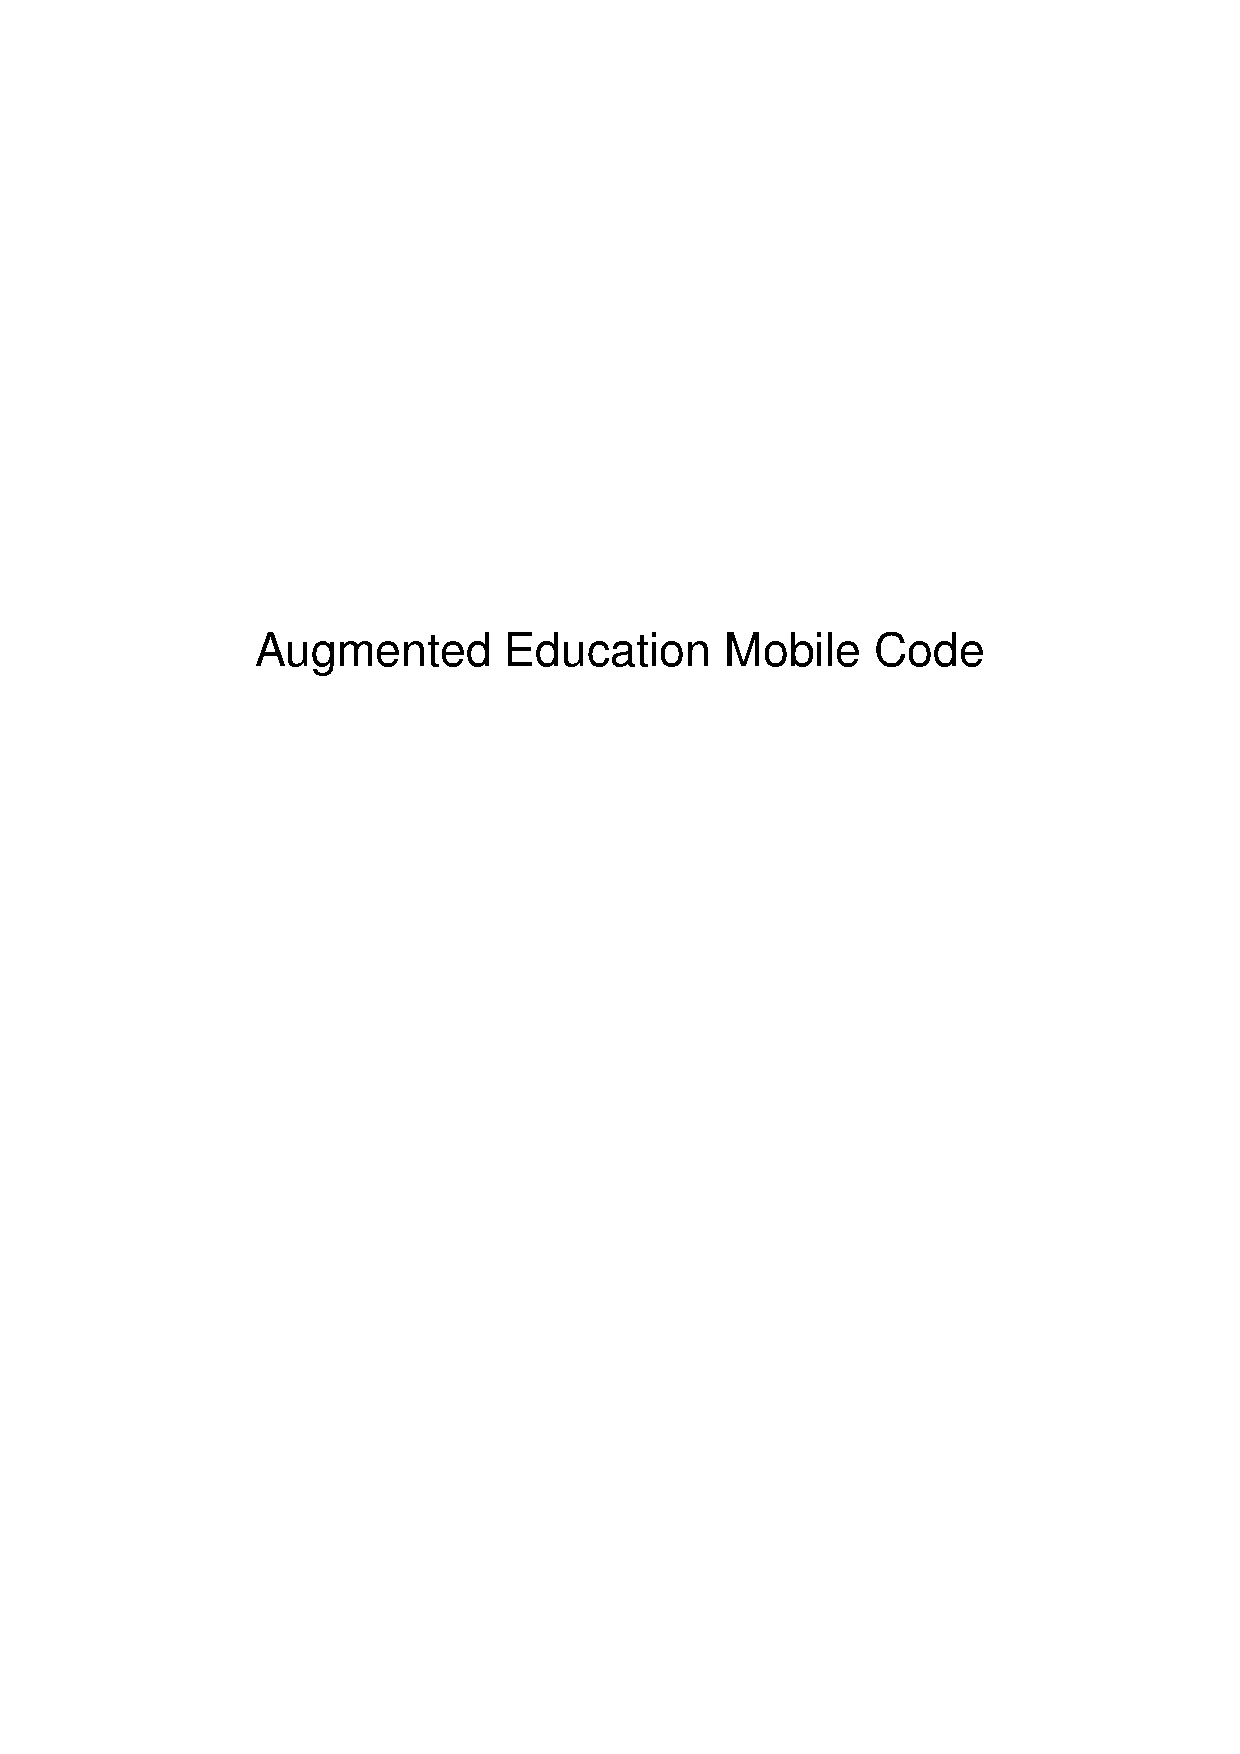
\includepdf[pages={1}, pagecommand=\section{Mobile Application}\hypertarget{mobile_CodeDocumentation}{\label{mobile_CodeDocumentation}\index{mobile_CodeDocumentation@CodeDocumentation}}]{CodeDocumentation/MobileCodeDoc}
\includepdf[pages={2-}]{CodeDocumentation/MobileCodeDoc}
  %% All tracks

% !TEX encoding = UTF-8 Unicode
% !TEX root = DesignDocument.tex

\chapter{Business Plan}

InTouch L.L.C. is a custom software solutions company owned and run by students directly involved in the development of Augmented Education. Included in this appendix is the InTouch L.L.C. business plan and financial projections directly associated with the development of the Augmented Education product.  

\includepdf[pages={1-33}]{InTouchLLCBusinessPlan.pdf}   %% Entrepreneur track only 
% % !TEX root = DesignDocument.tex


\chapter{Hardware Exploration}

A Microsoft HoloLens, Meta 2, and Oculus Rift were purchased by the client and available for testing and exploration via student status of developers. The following notes are observations made regarding these AR or VR hardware options.

\begin{description}
\item Microsoft HoloLens
	\begin{description} 
		\item Pros
		\begin{itemize}
			\item Screen sharing over wireless internet  
			\item Ability to record AR view and output to video
			\item Hardware independence
			\item Ability to statically place objects in environment
			\item Support for most AR file types
		\end{itemize}
	\end{description}
	\begin{description} 
		\item Cons
		\begin{itemize}
			\item Most expensive AR device on market
			\item Portability plus value creates concern of theft
			\item Limited AR display size
			\item Limited availability of applications and support
		\end{itemize}
	\end{description}
\item Meta 2
	\begin{description} 
	\item Pros
	\begin{itemize}
		\item Largest AR display size on market
		\item AR and VR capable
	\end{itemize}
\end{description}
\begin{description} 
	\item Cons
	\begin{itemize}
		\item Hardware dependent
		\item Limited availability of applications and support
	\end{itemize}
\end{description}
\item Oculus Rift
	\begin{description} 
	\item Pros
	\begin{itemize}
		\item Immediate availability of supplementary educational programs
		\item Most economic VR device (current market price of \$400)
		\item Intuitive controls
	\end{itemize}
\end{description}
\begin{description} 
	\item Cons
	\begin{itemize}
		\item VR only (no support for QR code use or real world visualizations)
		\item Hardware dependent
		
	\end{itemize}
\end{description}
\end{description}   %% Research track  only


\chapter{Supporting Materials}
\label{sec:support}

These are materials that we refer to in our documentation. It includes the 
mobile computing grant submitted by Dr. McGough and other professors from 
various departments at SD Mines.

\includepdf[pages={1-8}]{MobileComputingGrant2017.pdf}


% chapters in back matter don't have numbers, but they appear in the
% table of contents, and are numbered BM-X where X is the page number
% relative to where the back matter begins.
\backmatter

\end{document}
